\documentclass{article}
\usepackage{graphicx} % Required for inserting images
\usepackage{float}
\usepackage[table,xcdraw]{xcolor}
\usepackage{array}
\usepackage{spverbatim}

\begin{document}
\begin{figure}[t]
    
\includegraphics[scale=0.8]{logo_polimi.png}
    \centering
\end{figure}

\begin{titlepage}
    \newcommand{\HRule}{\rule{\linewidth}{0.5mm}}
    \center
	\textsc{\Large SOFTWARE ENGINEERING II}\\[0.5cm]
	
	\HRule\\[0.4cm]
	    {\huge \textsc{Students\&Companies - \\Design Document}}\\[0.4cm]
    \HRule\\[1.5cm]
	
	\begin{minipage}{1\textwidth}
		\begin{flushleft}
			\large
			\textit{Authors}\\
			Priuli \textsc{Elia}\\
			Viceconti \textsc{Veronica}\\
			Zuccoli \textsc{Marco}\\
		\end{flushleft} 
         \hspace*{\fill} 6 January 2025 \newline
         \hspace*{\fill} Version 1
	\end{minipage}
\end{titlepage}

\newpage
\tableofcontents
\newpage
\section{Introduction}
\subsection{Purpose}
This document presents all the information regarding the design and architectural choices made to develop the S\&C software, its component and how they interact with each other to satisfy the requirements listed in the RASD document.\newline
In addition information about the testing, integration and implementation phases are provided.

\subsection{Scope}
The S\&C application aims to solve the problem of matching university students with companies that offer internships. Moreover the students' universities can stop an internship if relevant complaints are received.\newline
Different types of users means different devices with different hardware and power limitation, running different operating systems. \newline
As a consequence, a lightweight application with a shared codebase is desirable.\newline
Given these constraints a 3-tier, web-based application, with a thin client is the best solution (to address the hardware/power limitation).\newline
In order to simplify the implementation, the notification system will be implemented via the Google Firebase CloudMessaging.   

\subsection{Definitions, Acronyms, Abbreviations}
\begin{itemize}
    \item DB: Database
    \item DBMS: Database Management System
    \item S\&C: Students\&Companies
    \item IOS: Iphone Operating System
    \item SOA: Service Oriented Architecture
    \item RASD: Requirements Analysis and Specification Document 
    \item HTTPS: Hypertext Transfer Protocol over Secure Socket layer 
\end{itemize}

\subsection{Revision History}
\begin{itemize}
    \item Version 1 (6/01/2025) : First release of the document
\end{itemize}

\subsection{Reference Documents}
\begin{itemize}
    \item previous RASD document
    \item Assignment RDD AY 2024-2025.pdf on the webeep page of the course
\end{itemize}

\subsection{Document Structure}
The rest content of this document is divided into the 6 sections below:\newline\newline
\textbf{Introduction}: In the first section, we outline the project’s purpose and aim, and also incorporates a glossary of abbreviations and definitions necessary for understanding the issue.\newline\newline
\textbf{Architectural Design}: the key components and their interaction are shown here. This section also explains the main design and architectural choices.\newline\newline
\textbf{User Interface Design}: in this section are presented some mockups of the S\&C interfaces.\newline\newline
\textbf{Requirements Traceability}: Here is shown the mapping between requirements and design elements.  \newline\newline
\textbf{Implementation, Integration and Test plan}: Order in which you plan to implement subsystems and components as well as plan of the integration and test of the integration.\newline\newline
\textbf{Effort Spent}: here is explained the individual contributions of each team member in creating this document.\newline\newline
\textbf{References}: All the referenced documents used to draft this one. 

\section{Architectural Design}

\subsection{Overview}

We have decided to develop the software through a WebApp and consequently to implement a 3-tier architecture, because: 
\begin{enumerate}
    \item On the client side, a light and non-constant computation is required. 
    \item Exploitation of existing protocols such as HTTPS, servlets, DBMS, and REST APIs for a modular and rapid implementation.
    \item Maintainability: The application is easily maintainable and updatable. 
    \item Platform independent: it is not necessary to write different applications for different devices (PC, Mac, Android, iOS ...). By using web technologies, a single codebase that is accessible and usable by the various browsers already on the market and widely used is sufficient. 
    \item Scalability: as the number of users increases, it is possible to scale the infrastructure by adding more servers in parallel (scale out) to handle more requests simultaneously. 
    \item Reusability: the logic, for example of matchmaking, can also be reused for future projects. 
    \item Greater throughput: increases the ability to perform more work in parallel, reducing user wait time and increasing the usability of the WebApp. 
\end{enumerate}
The first tier is an interface level with a thin client, the second is the S\&C server which manages both the web service and the actual computation (including match calculation), and finally, there is a server that hosts the DBMS and the actual database.  

\begin{figure}[H]
    \centering
    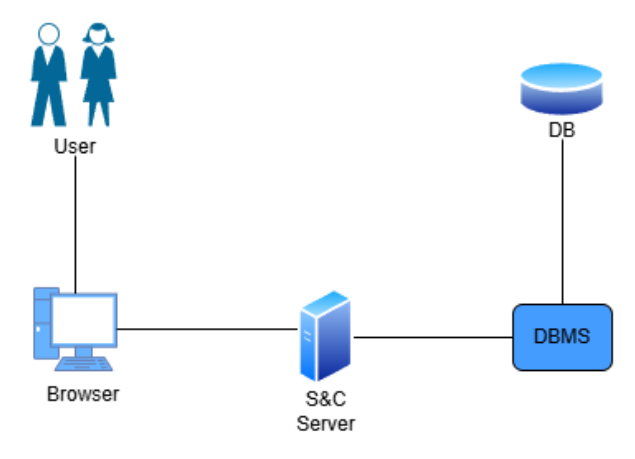
\includegraphics[width=0.5\linewidth]{overview.png}
    \caption{Three-tier architecture}
    \label{fig:enter-label}
\end{figure}
\subsection{Component View}
\begin{figure}[H]
    \centering
    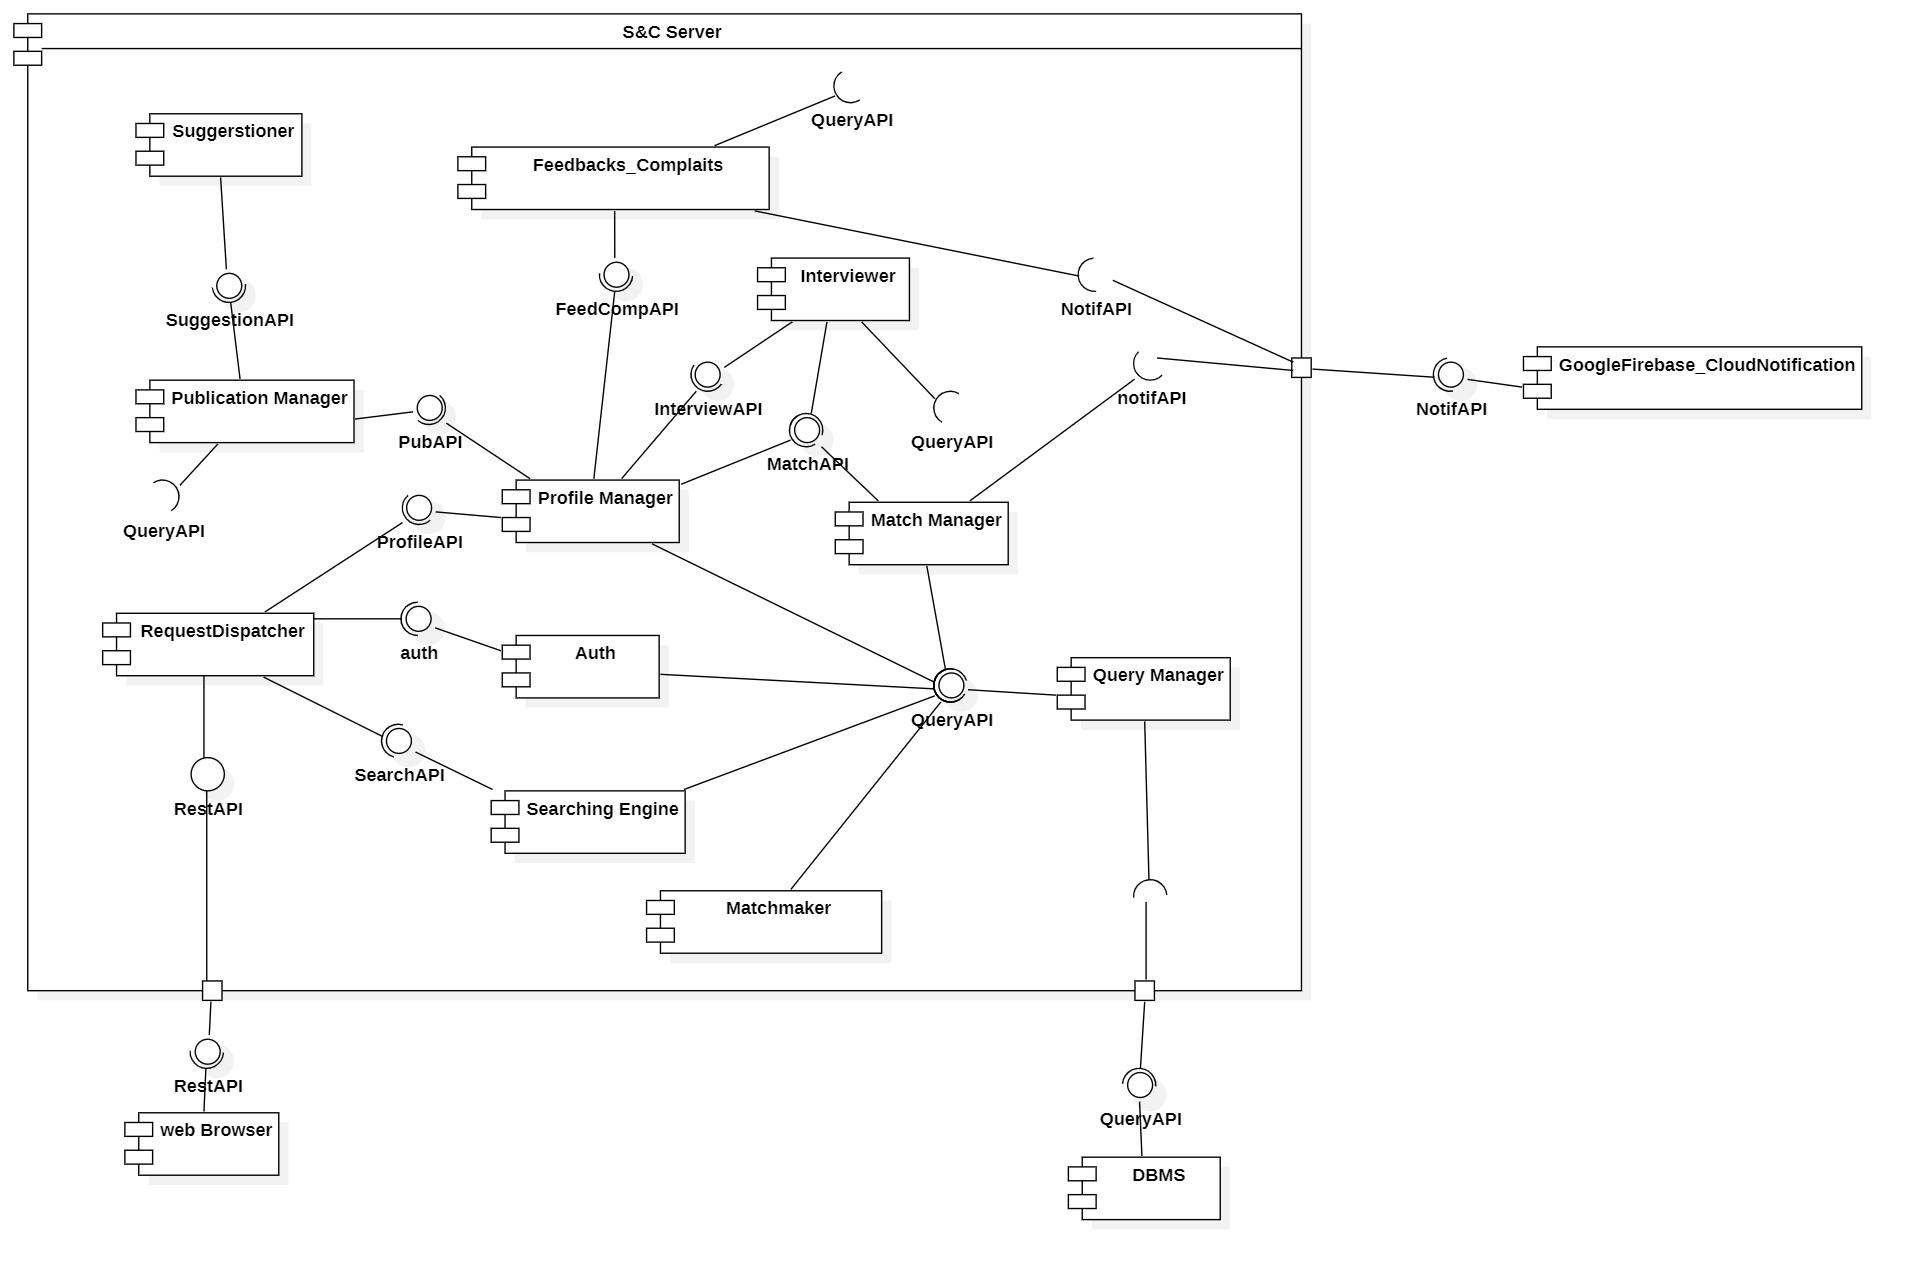
\includegraphics[width=1\linewidth]{ComponentDiagram.jpg}
    \caption{Component view}
    \label{fig:enter-label}
\end{figure}

\subsubsection{Request Dispatcher}
This component is responsible for receiving various requests from the web app and has the task of routing them to the various other components based on the specific request. For this reason, it interacts with Profile Manager, Auth, and Searching Engine. 

\subsubsection{Profile Manager}
This component allows universities to manage complaints, enabling the removal of ongoing internships, if necessary. \newline Furthermore, it communicates with other components that manage the publication of students and companies, feedback/complaints, and interviews, and with the Query Manager to obtain the data requested by the user.

\subsubsection{Publication Manager}
This component is responsible for managing the publications of students and companies. It allows these users to view existing publications, as well as create, modify, and delete them.  \newline
To carry out these activities, the component communicates with the Query Manager to obtain the necessary data and make the corresponding changes. It also communicates with the Suggestioner component to allow users who want to improve their publication to receive suggestions. 

\subsubsection{Feedbacks\_Complaints}
This component is responsible for managing user feedback and complaints. It then communicates with the Query Manager to insert or obtain the necessary data. 

\begin{figure}[H]
    \centering
    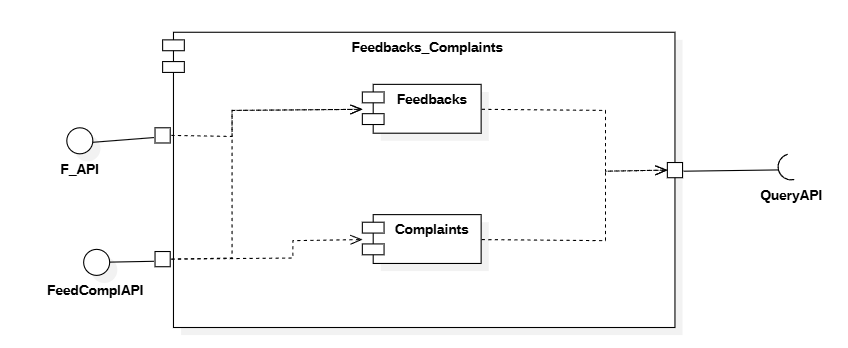
\includegraphics[width=1\linewidth]{FeedComplComponent.png}
    \caption{Component Feedbacks\_Complaints}
    \label{fig:enter-label}
\end{figure}

The sub-component Feedbacks manages everything related to user feedback, including creation and visualization, as well as the use of this data to allow other components to create suggestions. The sub-component Complaints manages everything related to user complaints, including creation and visualization. 

\subsubsection{Interviewer}
This component is responsible for managing the interviews conducted with the various students accepted by companies. It allows the creation of the form, formatting it, recording the students' responses, and saving everything. Furthermore, following the interviews, it communicates with the Match Manager to handle the acceptance or rejection of the students. 

\subsubsection{Match Manager}
This component is responsible for managing the matches found by the MatchMaker component. It allows viewing all matches created for a particular user and accepting or rejecting them. Additionally, it communicates with the Query Manager to request the necessary data and with the GoogleFirebase\_CloudNotification API to send notifications of new matches and acceptance/rejection to various users or new complaints to universities. 

\subsubsection{Auth}
This component is responsible for managing user registration and authentication. It is therefore composed of two sub-components, Registrator and Authenticator. 

\begin{figure}[H]
    \centering
    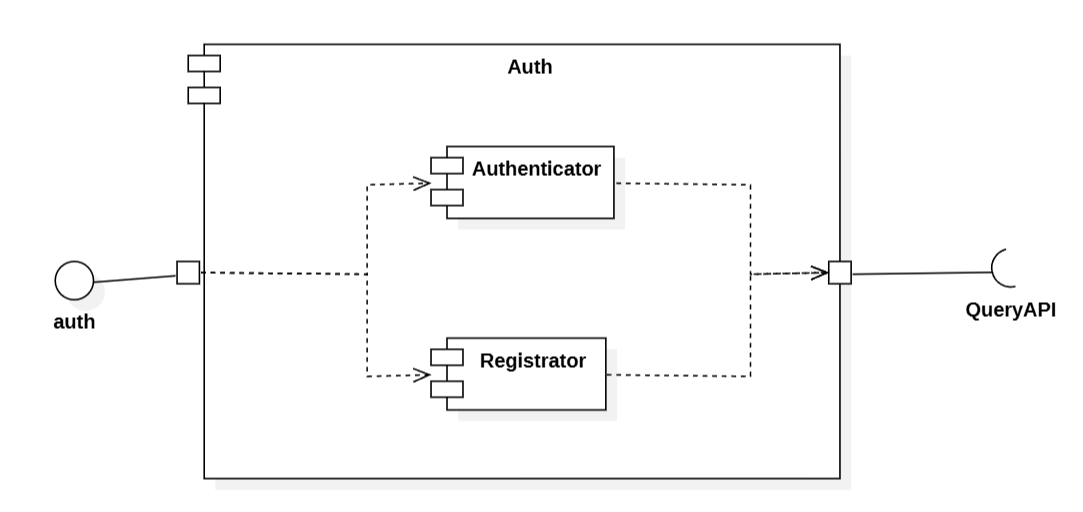
\includegraphics[width=1\linewidth]{AuthComponent.png}
    \caption{Component Auth}
    \label{fig:enter-label}
\end{figure}

The sub-component Authenticator is responsible for managing user authentication, whether it is a Student, Company, or University, by checking the data and, if possible, allowing access to the system. The sub-component Registrator is responsible for managing user registration, whether it is a Student, Company, or University, by checking the data and communicating with the Query Manager to update the database. 

\subsubsection{Searching Engine}
This component is responsible for managing the searches performed in the system by users (students can search for and view company profiles, and companies can request to view the profile of a specific user with whom they have a match). It interacts with the Query Manager to obtain the data requested by the user. Additionally, this component is responsible for searching and making visible to students all possible internships, so they can manually search for the one that interests them. 

\subsubsection{MatchMaker}
This component is responsible for finding matches between companies and students, using different levels of sophistication, thanks to communication with the Query Manager to obtain all the data useful for creating matches (all companies, all students, ...). 

\subsubsection{Query Manager}
This component is responsible for interfacing with the external DBMS component through queries that request specific data to be extracted from the database. 

\subsubsection{Suggestioner}
This component is responsible for enabling users to improve their visibility thanks to some suggestions (for CVs and internships) created by this component and allowing the users to visualize them, through the interface, by the Publication Manager component.

\subsubsection{GoogleFirebase\_CloudNotification}
This is an external component to the system that handles the notifications sent from the system to users (new matches, accepted or rejected matches, new complaints). 

\subsection{Deployment View}
\begin{figure}[H]
    \centering
    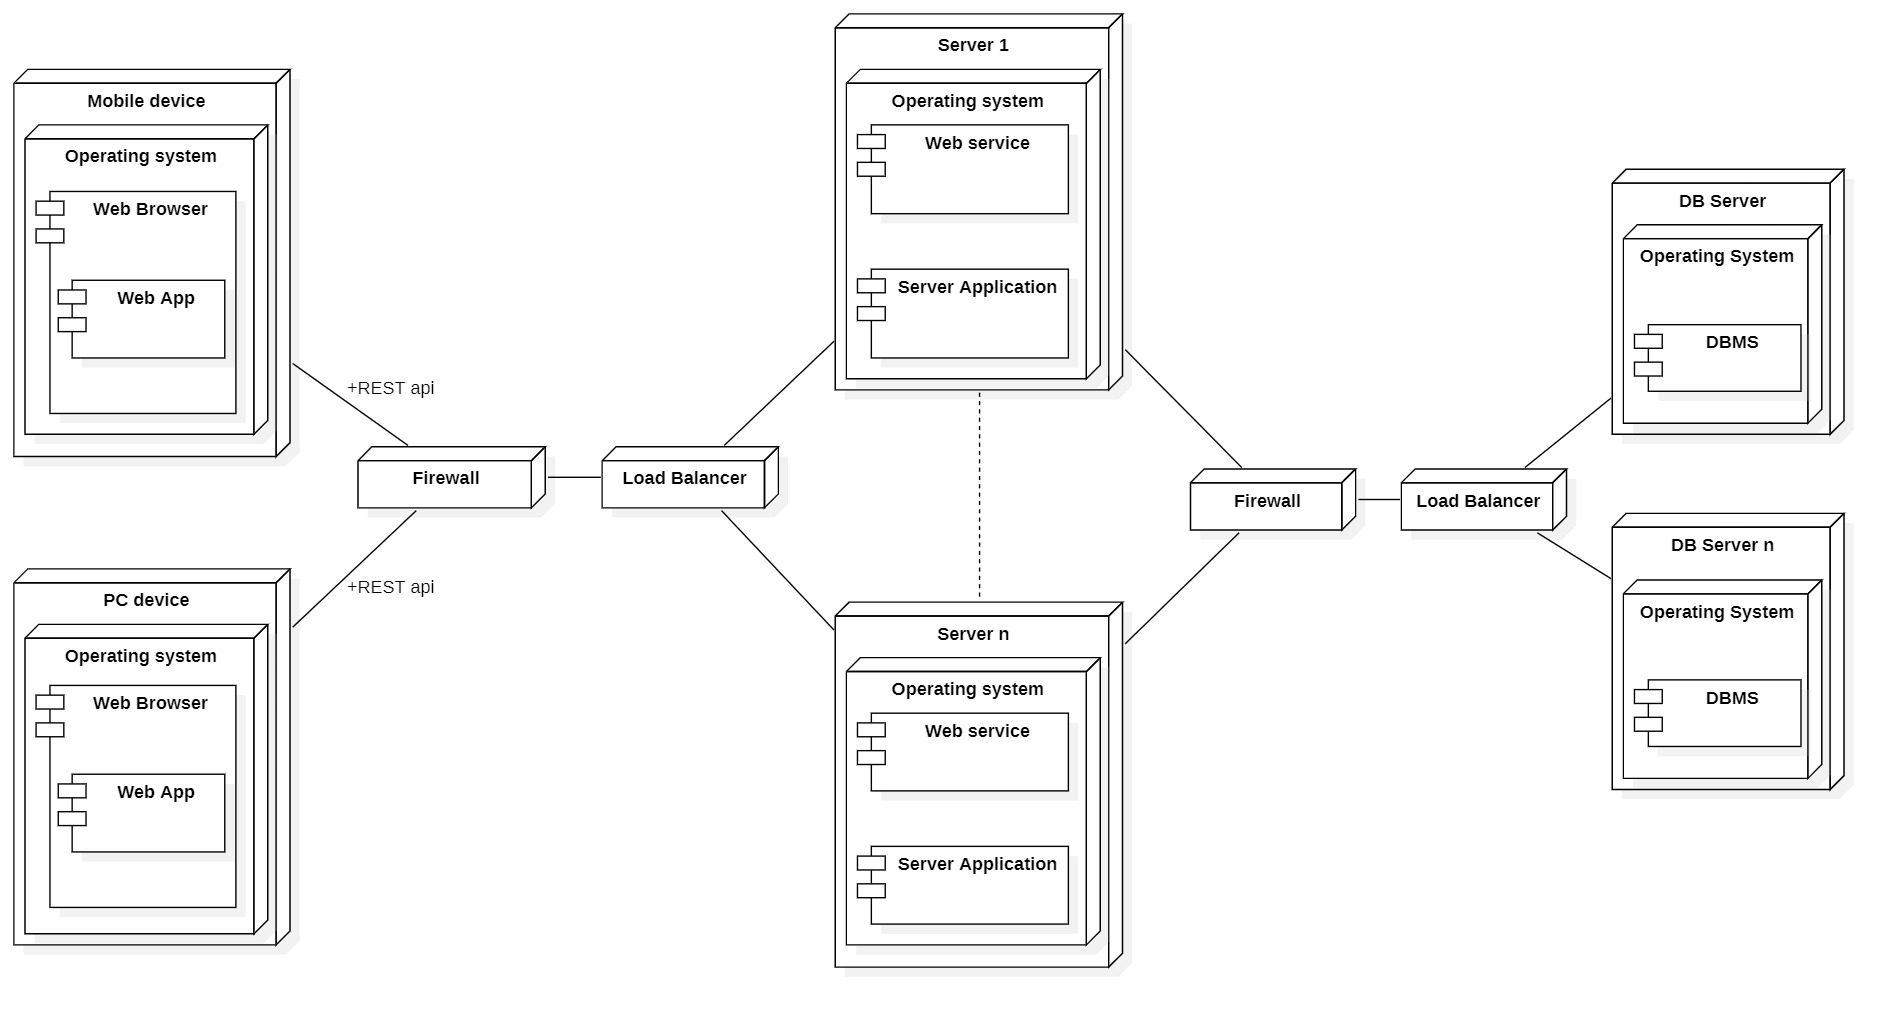
\includegraphics[width=1\linewidth]{DeploymentDiagram.jpg}
    \caption{Three-tier architecture}
    \label{fig:enter-label}
\end{figure}

\begin{itemize}
    \item \textbf{Mobile/Pc Device} : the devices user could use to access the service. Every device runs on its operating system and executes a web browser. It then connects with the web server via Rest APIs. They host the presentation layer.  
    \item \textbf{firewall} : This component prevents the system to be attacked 
    \item \textbf{load balancer} : It forwards the requests to different servers to distribute the workload 
    \item \textbf{Server 1..n} : The web servers that host the logic layer of the 3-tier architecture. It proved the S\&C service to all the clients
    \item \textbf{DB servers} : the DB server handles data storage, retrieval, and management, acting as the middle tier between the application server and the data. It ensures efficient access to data and supports queries from the application layer.
\end{itemize}

\subsection{Runtime View}
In this section we are going to illustrate all the sequence diagrams that are useful for understanding the interactions within different components.

\subsubsection{Login}
\begin{figure}[H]
    \centering
    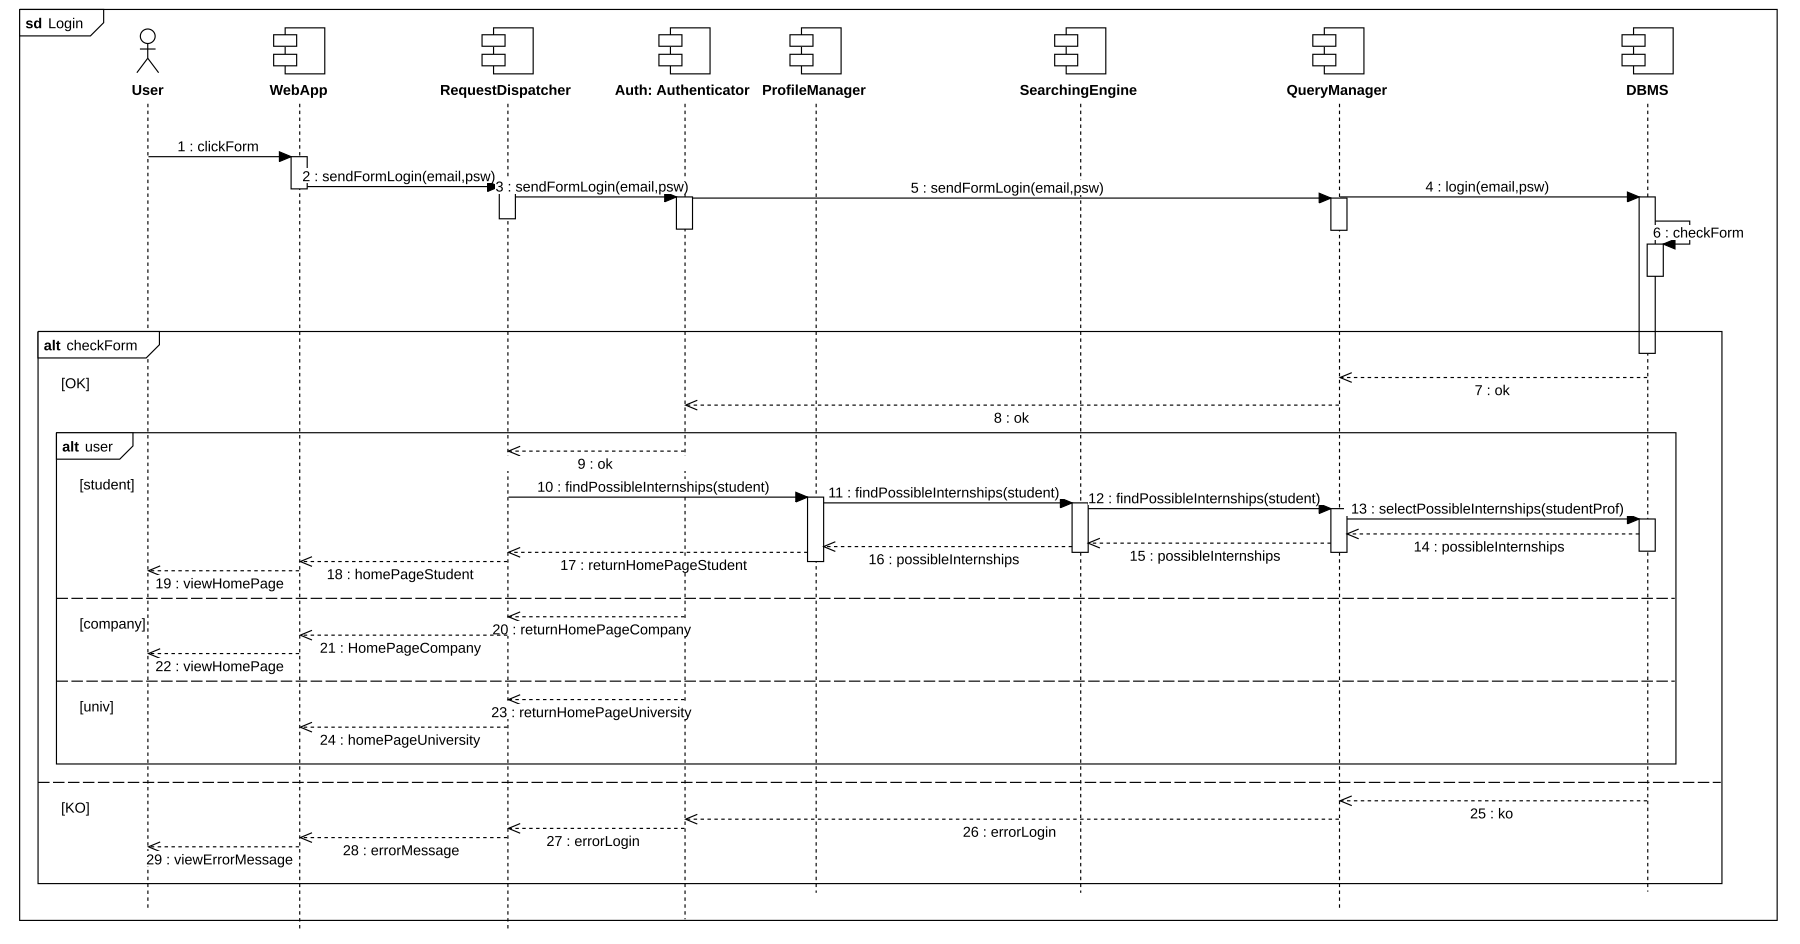
\includegraphics[width=1\linewidth]{SequenceDiagram/LoginSD.png}
    \caption{Login Sequence Diagram}
    \label{fig:enter-label}
\end{figure}
This sequence diagram allows the user to log in, thus entering the application. To log in, the user must correctly enter their email and password, so that the system allows them to access their homepage. If the user logging in is a student, then the system, through the SearchingEngine component, searches for all company internships and makes them visible on the student's homepage. 

\subsubsection{Registration}
\begin{figure}[H]
    \centering
    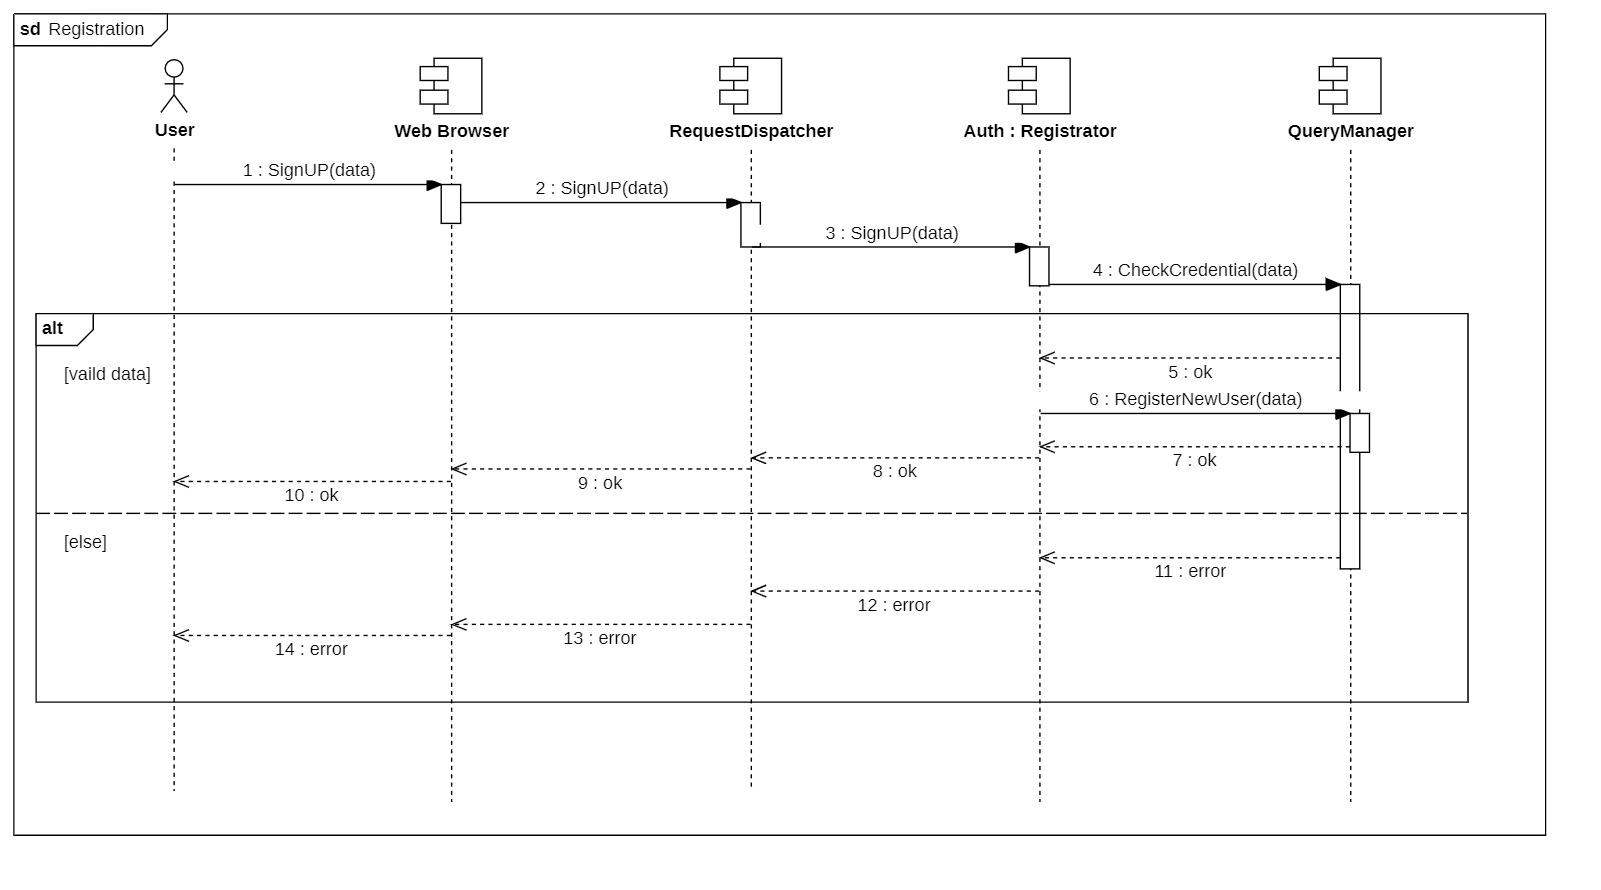
\includegraphics[width=1\linewidth]{SequenceDiagram/Registration.jpg}
    \caption{Registration Sequence Diagram}
    \label{fig:enter-label}
\end{figure}
The sequence diagram above describes  the event's flow that leads to the registration of a new user. The flow starts with the user who provides its information to the web browser. The information is then forwarded through the displayed components and finally reaches the QueryManager. Here the email's validity is checked and a proper answer is forwarded back to the user 

\subsubsection{CV \& Preferences publication}

\begin{figure}[H]
    \centering
    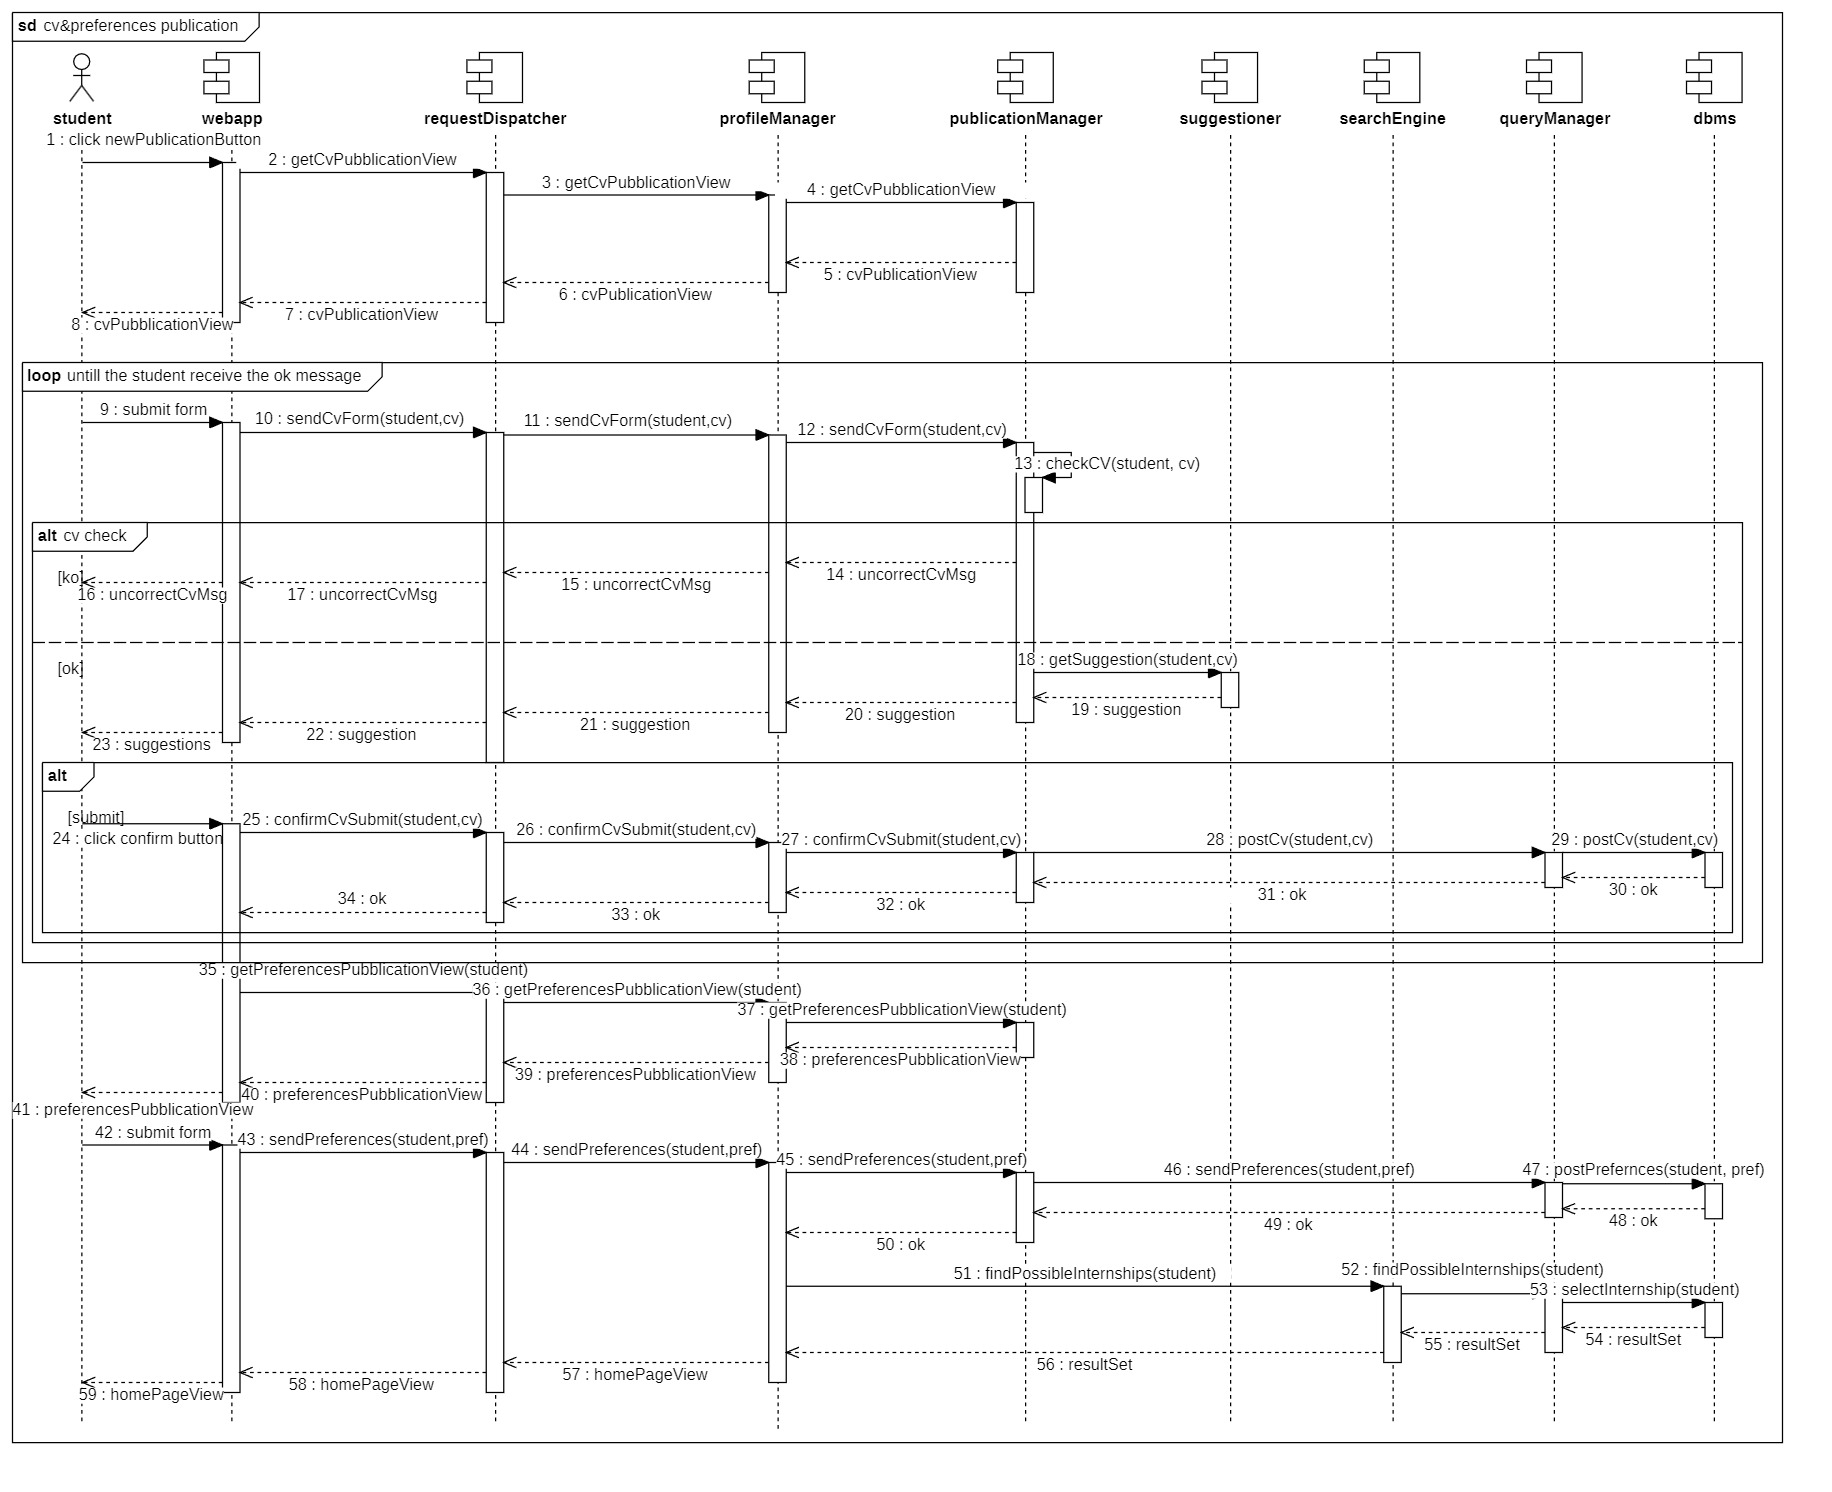
\includegraphics[width=1\linewidth]{SequenceDiagram/cv&preferences publication.jpg}
    \caption{CV \& Preferences publication Sequence Diagram}
    \label{fig:enter-label}
\end{figure}
This sequence diagram allows the student to upload their CV, with the possibility of accepting the application's suggestions, and publishing it with their preferences. 

\subsubsection{Manage CV}

\begin{figure}[H]
    \centering
    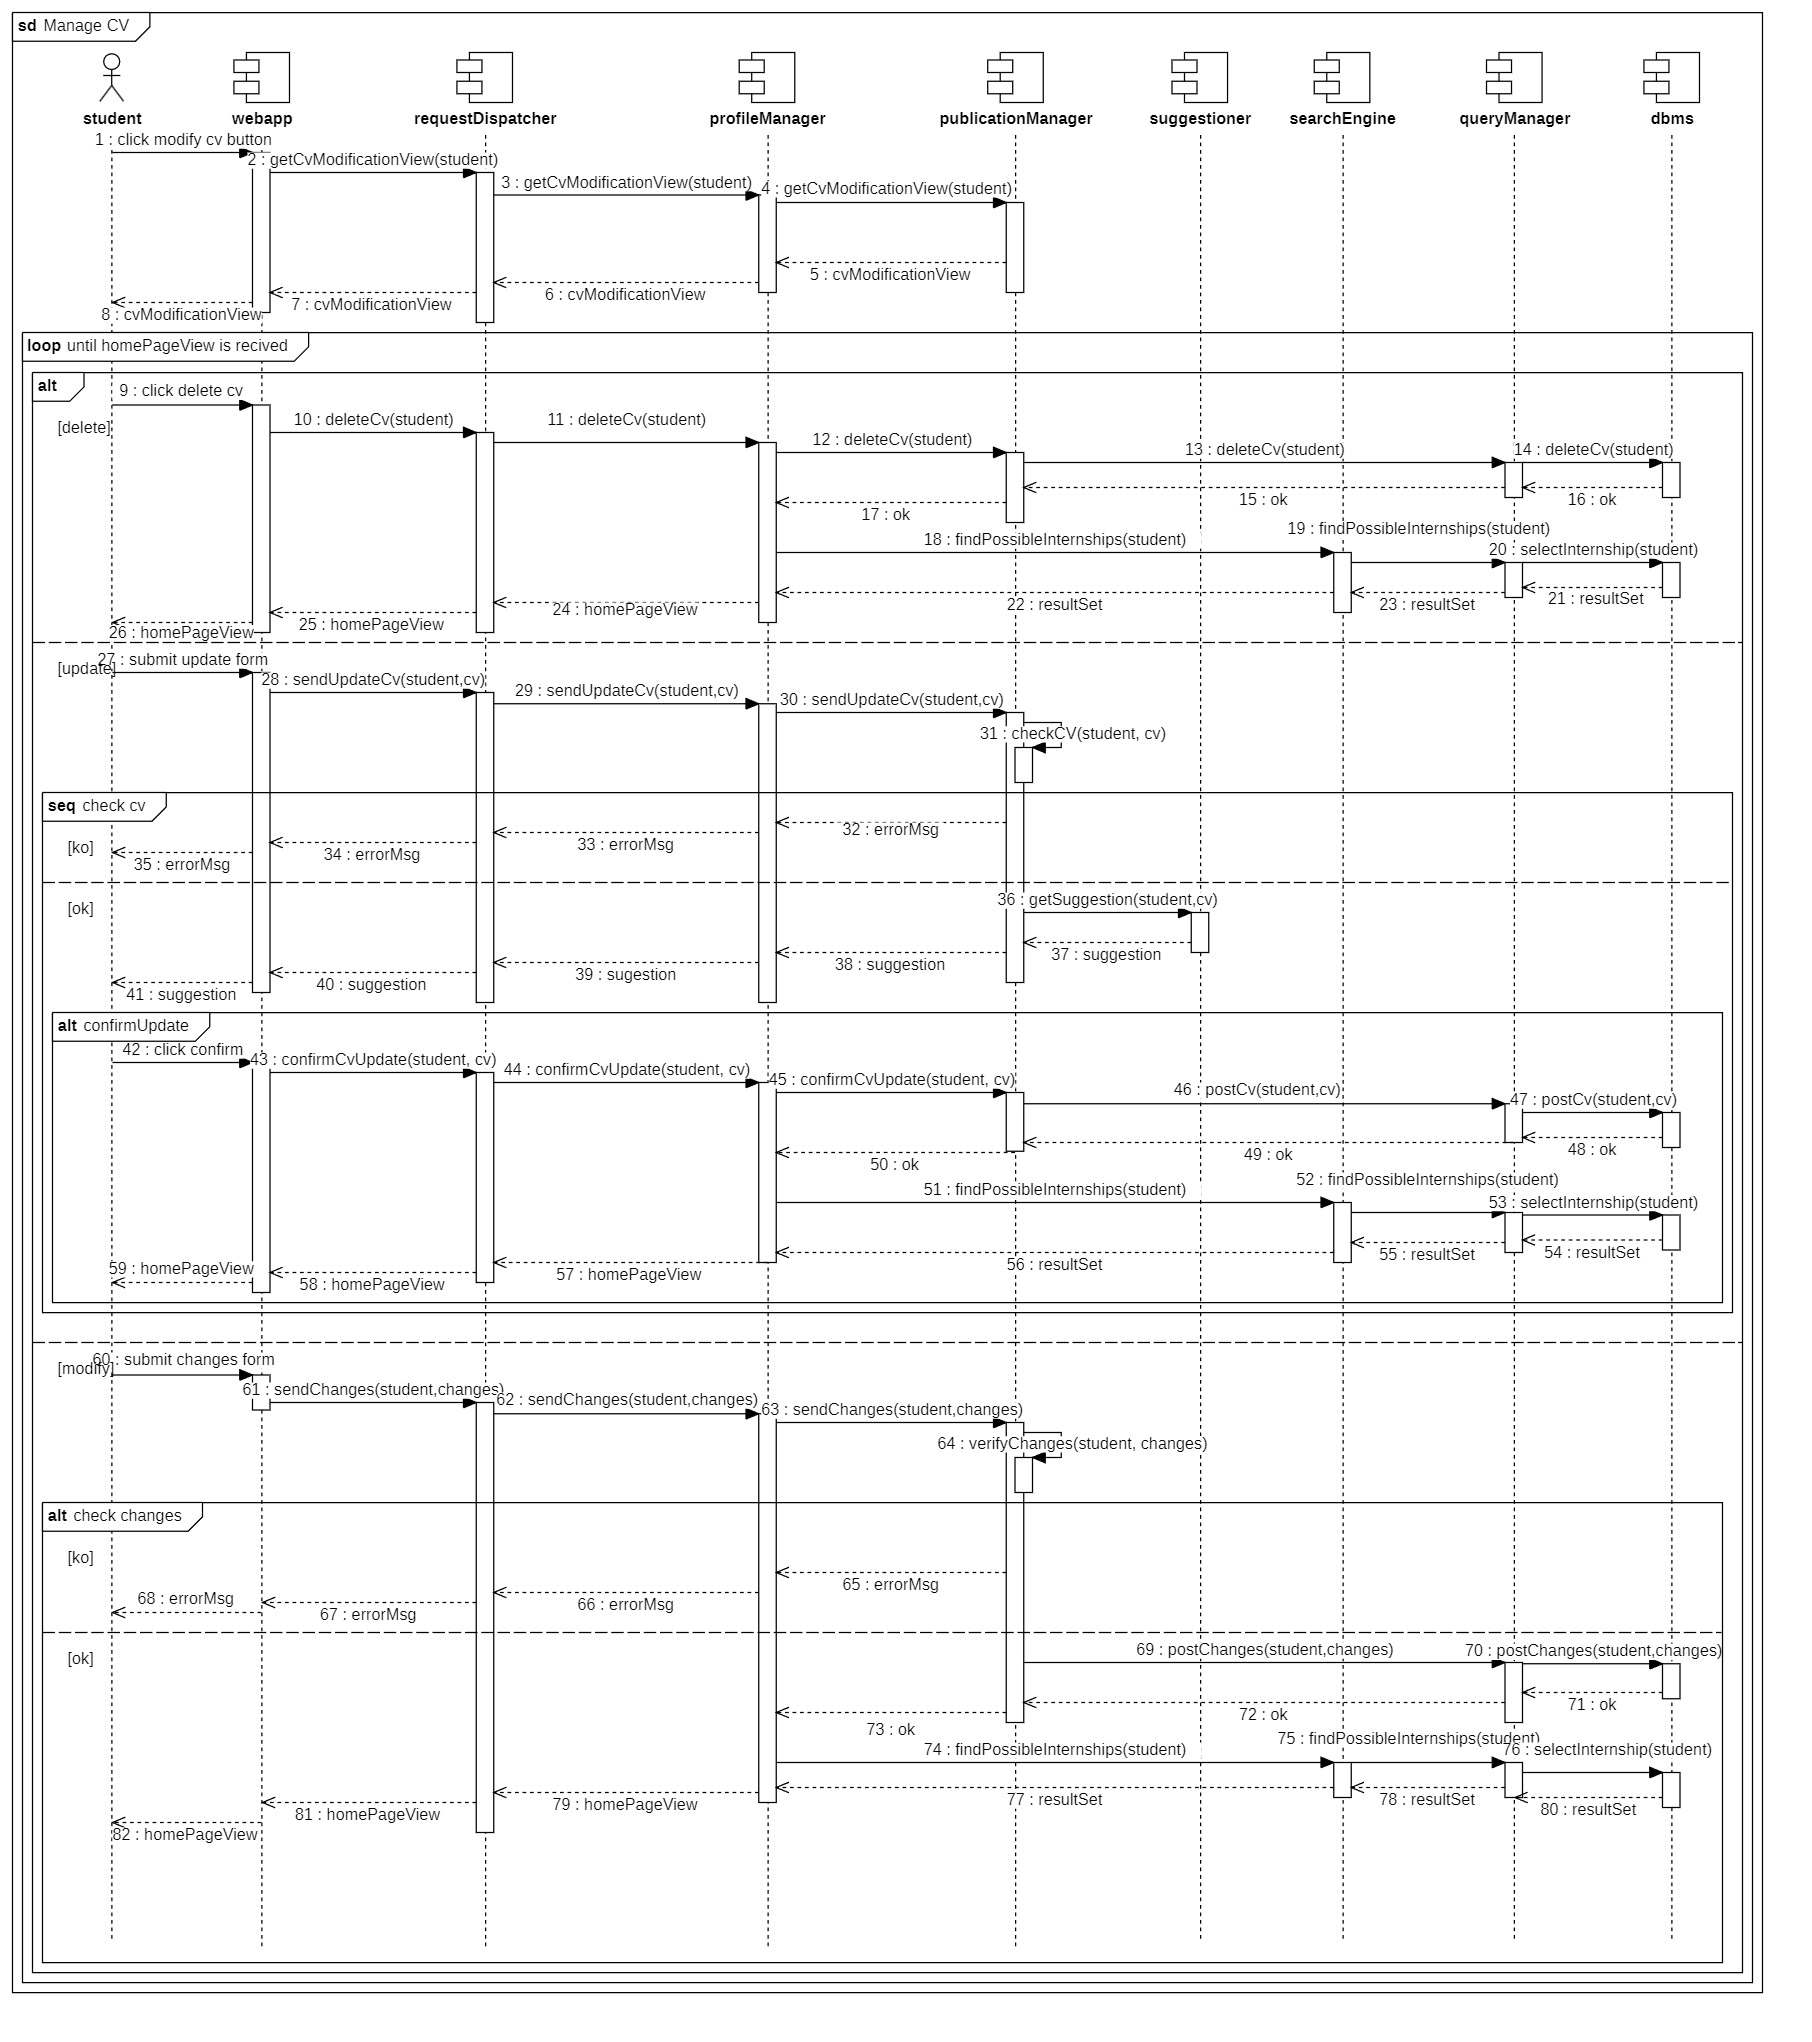
\includegraphics[width=1\linewidth]{SequenceDiagram/Manage CV.jpg}
    \caption{Manage CV Sequence Diagram}
    \label{fig:enter-label}
\end{figure}
This sequence diagram allows the student to modify, update, or delete their CV. 
The student after receiving the modification page can choose which operation performs, after the end of the operation the student will be redirect to the home page.

\subsubsection{Manage student publication}

\begin{figure}[H]
    \centering
    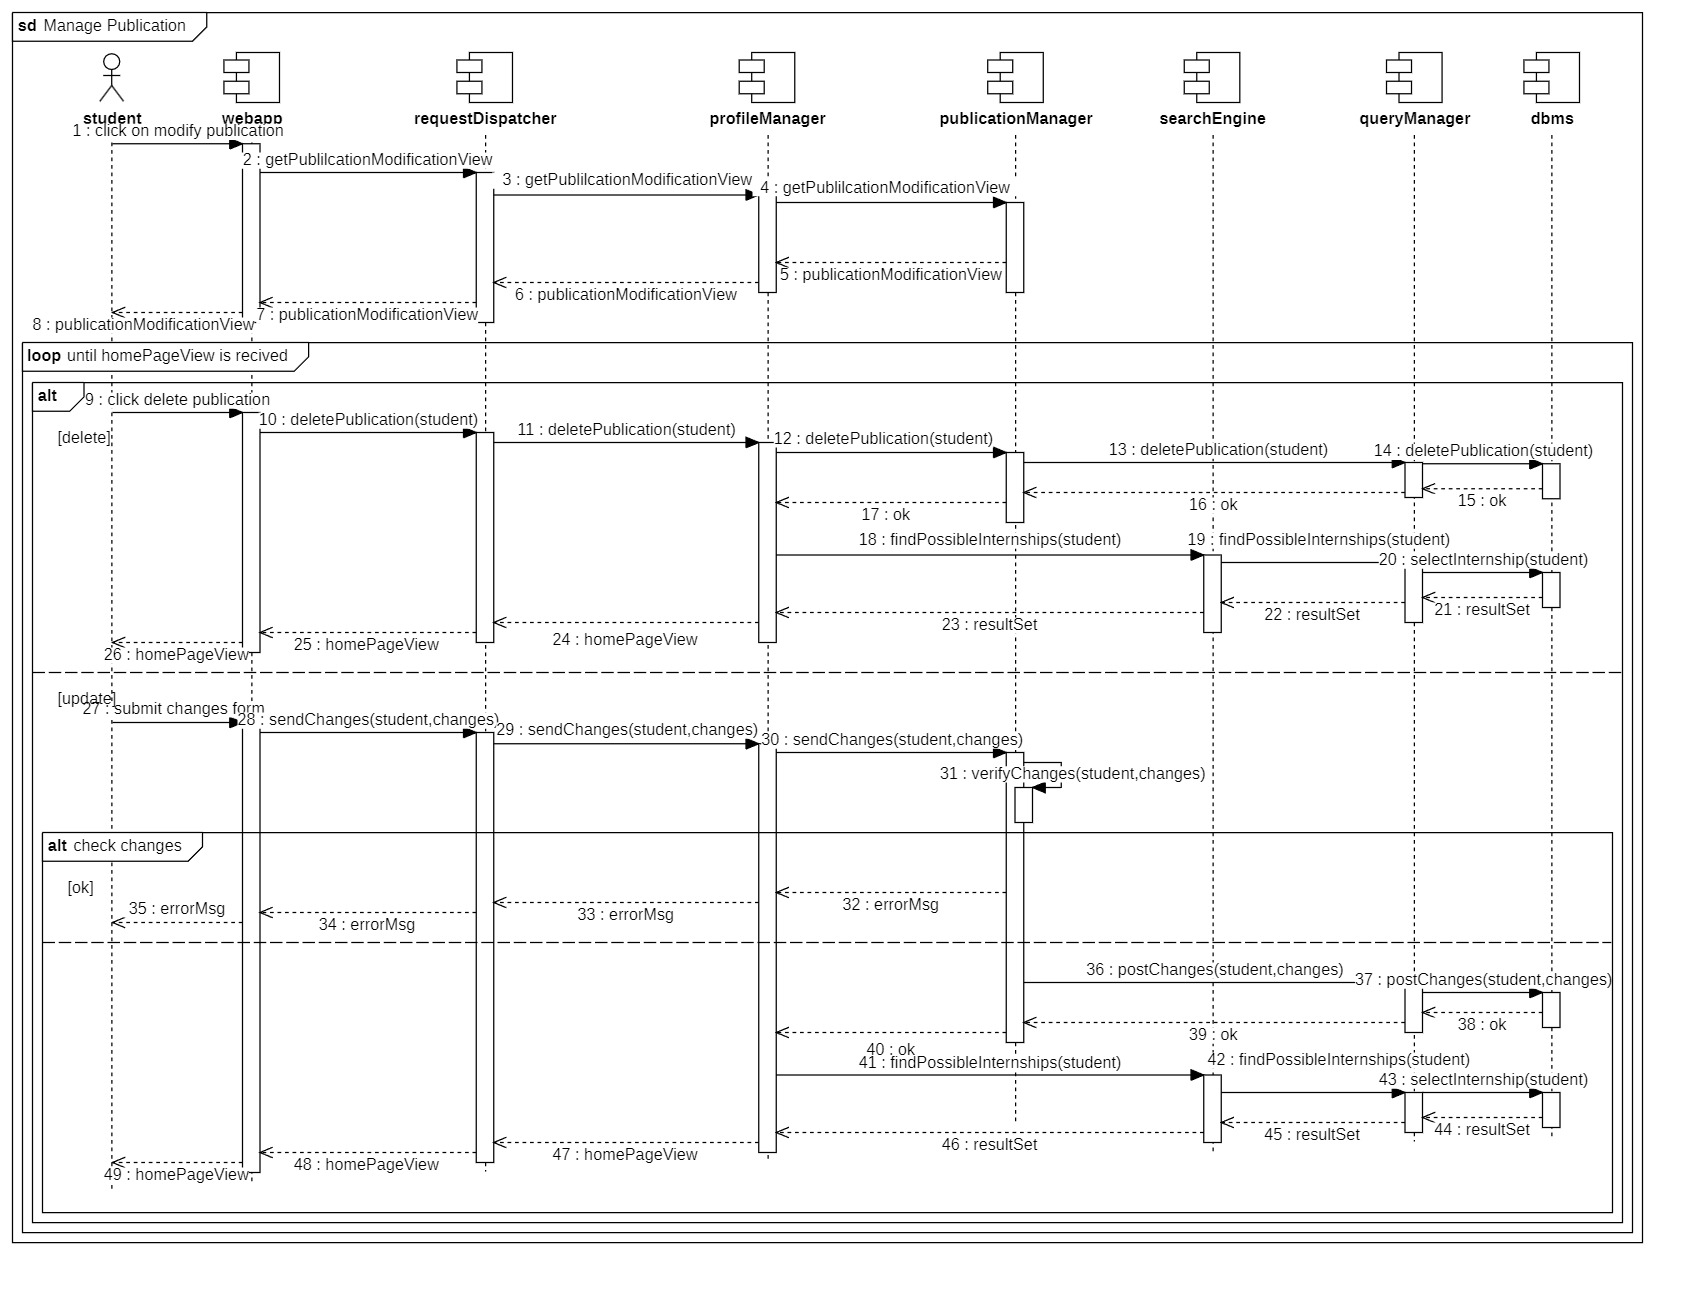
\includegraphics[width=1\linewidth]{SequenceDiagram/Manage Publication.jpg}
    \caption{Manage student publication Sequence Diagram}
    \label{fig:enter-label}
\end{figure}
This sequence diagram allows the students to modify or delete their publication. 
The student after receiving the modification page can choose which operation performs, after the end of the operation the student will be redirect to the home page.

\subsubsection{Search Internship}

\begin{figure}[H]
    \centering
    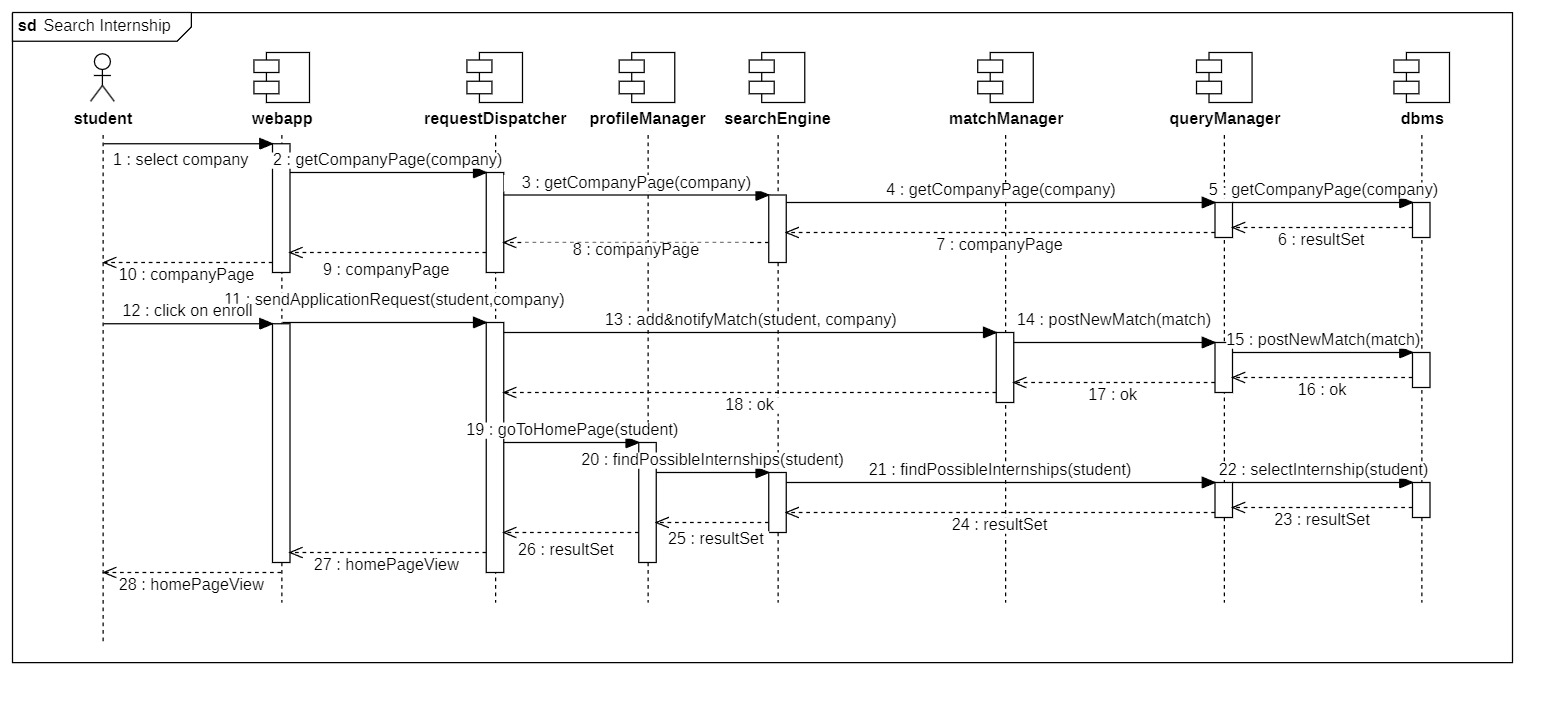
\includegraphics[width=1\linewidth]{SequenceDiagram/Search Internship.jpg}
    \caption{Search Internship Sequence Diagram}
    \label{fig:enter-label}
\end{figure}
This sequence diagram allows the user to select a company and enroll, the system will create a new match and will send a notification to the company.
\subsubsection{AcceptDeclineInternships}
\begin{figure}[H]
    \centering
    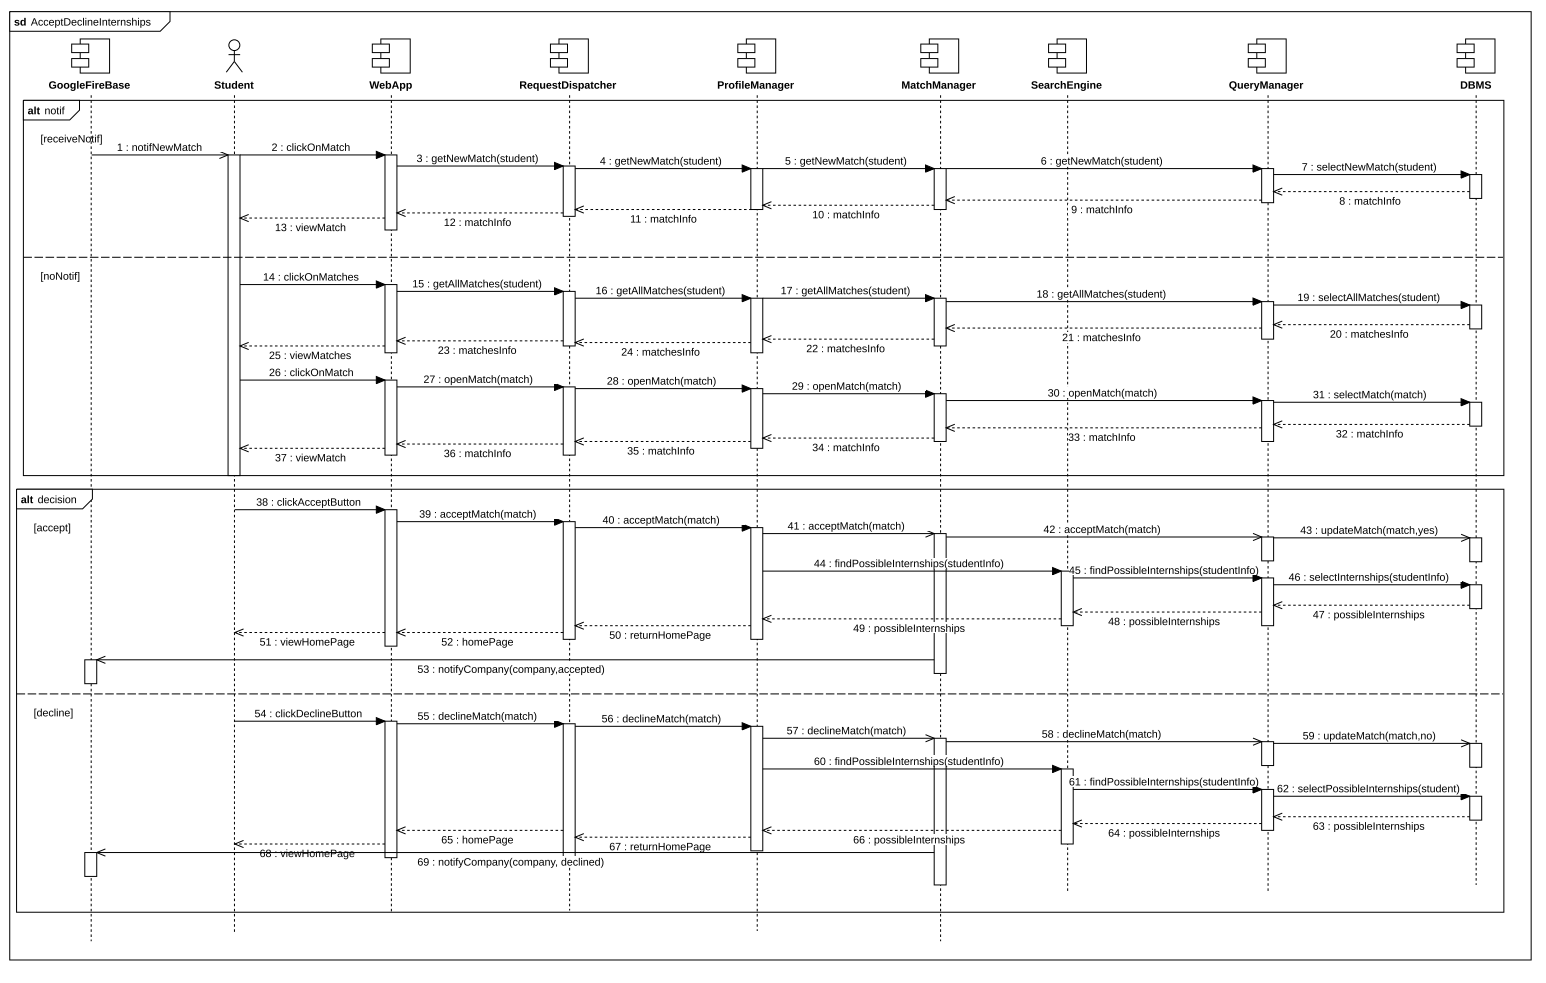
\includegraphics[width=1\linewidth]{SequenceDiagram/AccDeclInterSD.png}
    \caption{AcceptDeclineInternship Sequence Diagram}
    \label{fig:enter-label}
\end{figure}
This sequence diagram allows students to accept or reject a new match. The interaction can begin either via notification, where the student directly opens the found match, or manually, within their profile, they access the matches, select one, and decide whether to accept or reject it. Following the student's choice, the corresponding company is notified.

\subsubsection{PublishComplain student}
\begin{figure}[H]
    \centering
    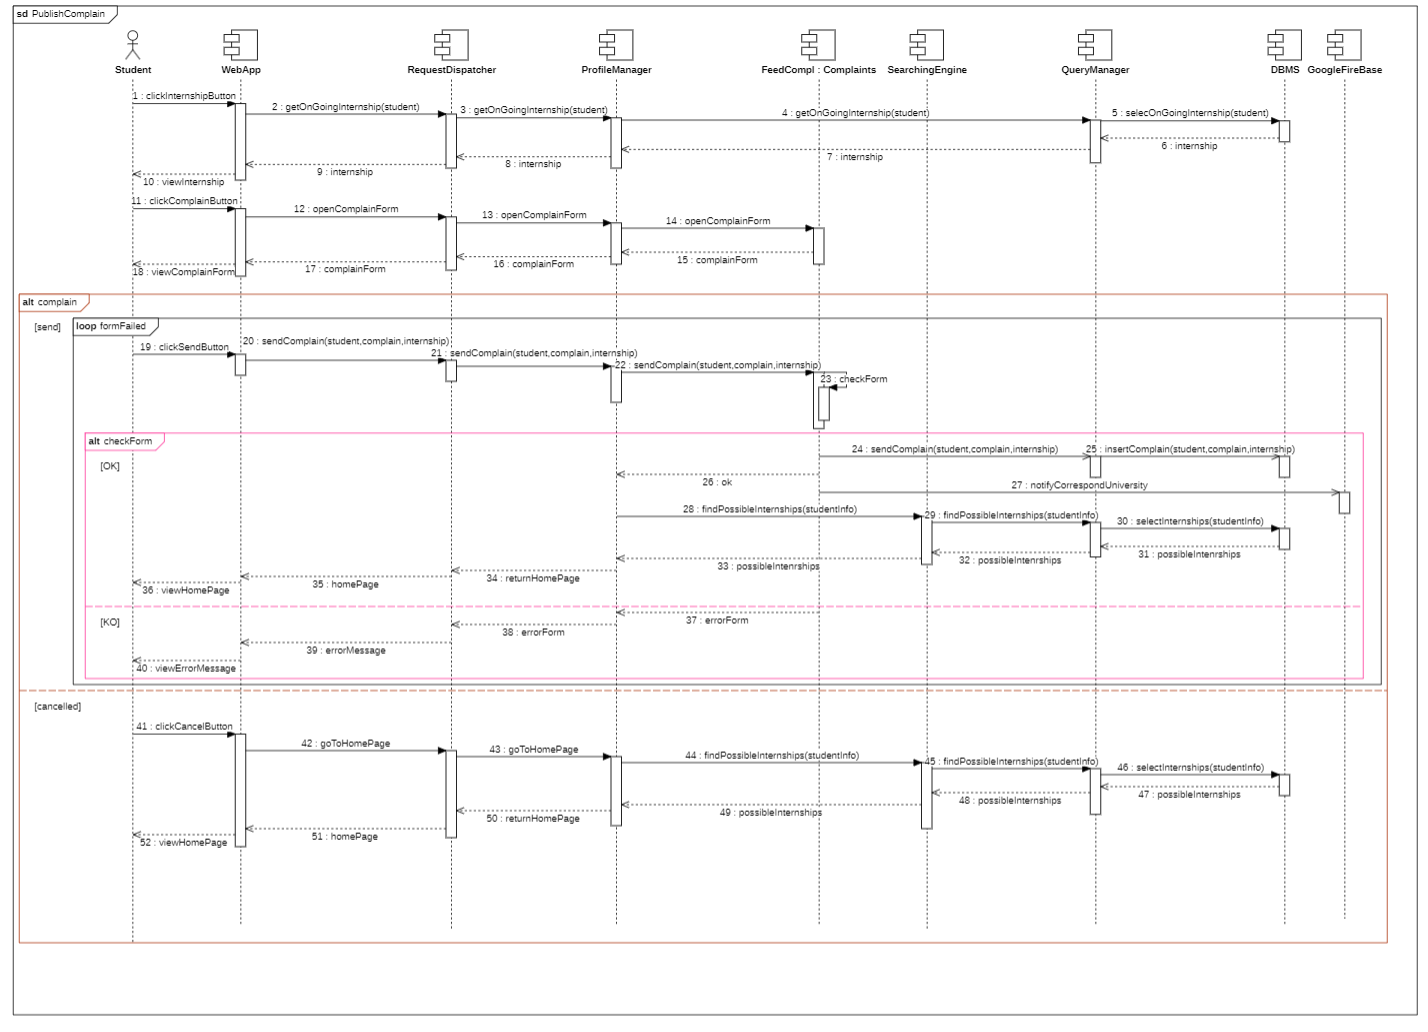
\includegraphics[width=1\linewidth]{SequenceDiagram/PublComplSD.png}
    \caption{PublishComplain Sequence Diagram}
    \label{fig:enter-label}
\end{figure}
This sequence diagram allows the student to interact with the system to write a complaint about their current internship. To do this, they first request the internship data and the corresponding form to write the complaint, and then either submit it or delete it if they change their mind. Until the form is correctly submitted, the system returns an error message. The system then notifies the corresponding university of the new complaint. 

\subsubsection{PublishFeedBack student}
\begin{figure}[H]
    \centering
    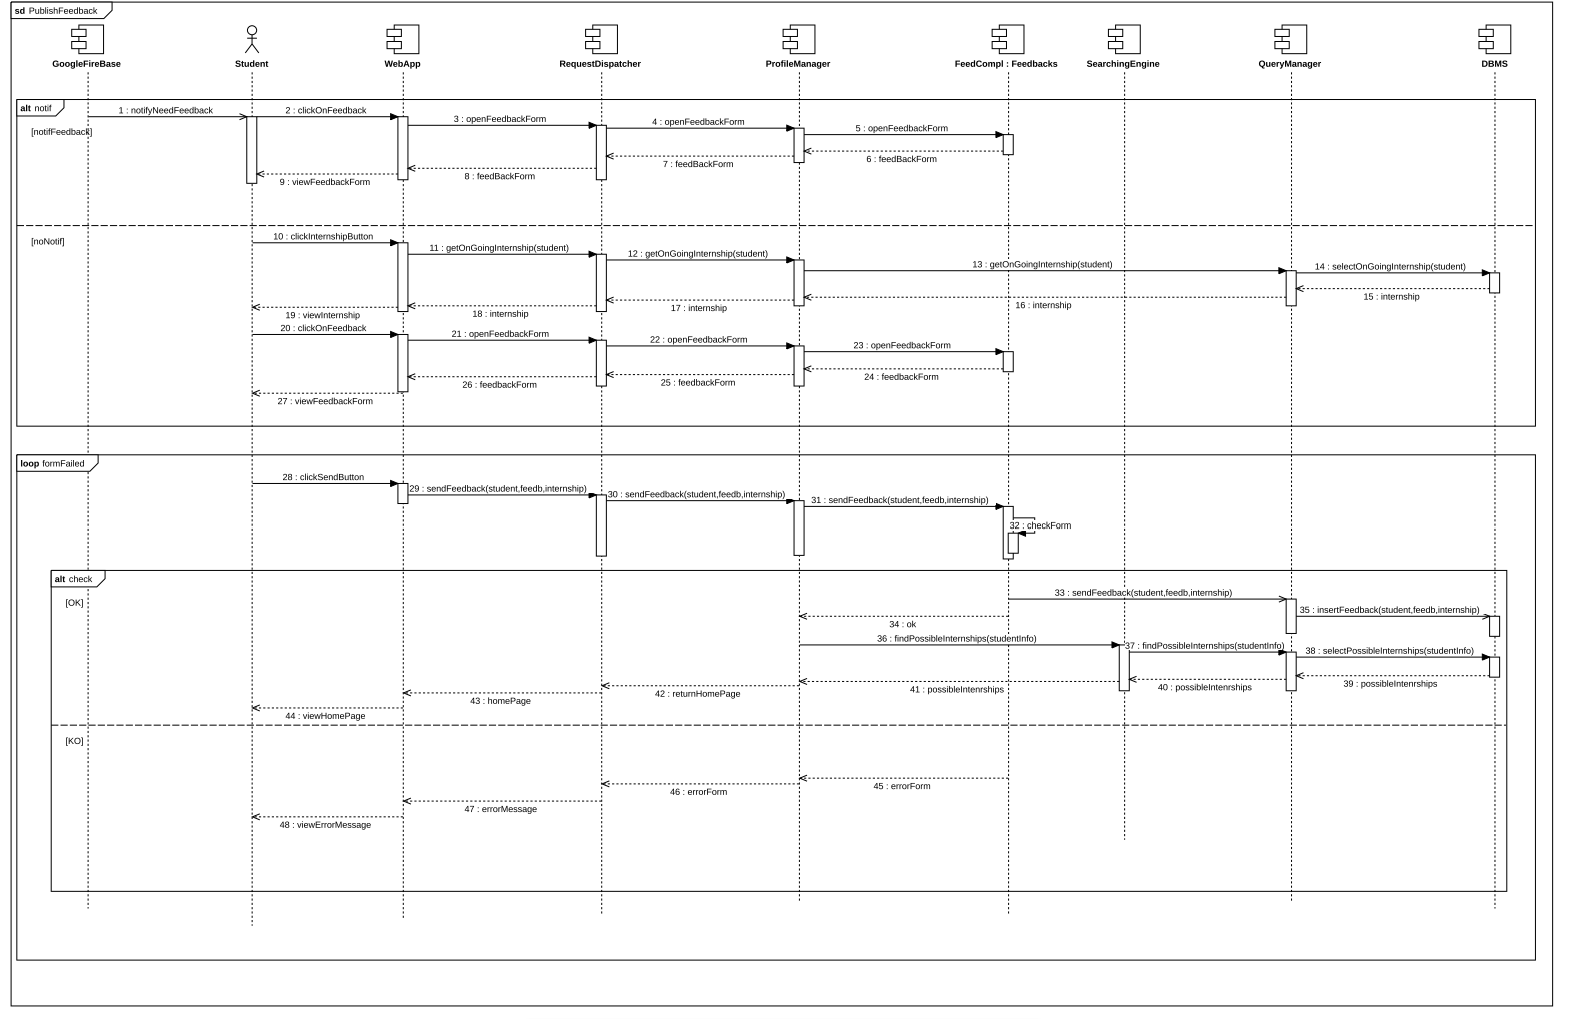
\includegraphics[width=1\linewidth]{SequenceDiagram/PubFeedSD.png}
    \caption{PublishFeedBack Sequence Diagram}
    \label{fig:enter-label}
\end{figure}
This sequence diagram allows the student to interact with the system to insert feedback at the end of their internship. To do this, they either receive a notification and open the form to write and submit the feedback, or they can manually open the internship and write the feedback. Until the form is correctly submitted, the system returns an error message.

\subsubsection{ManageComplains university}
\begin{figure}[H]
    \centering
    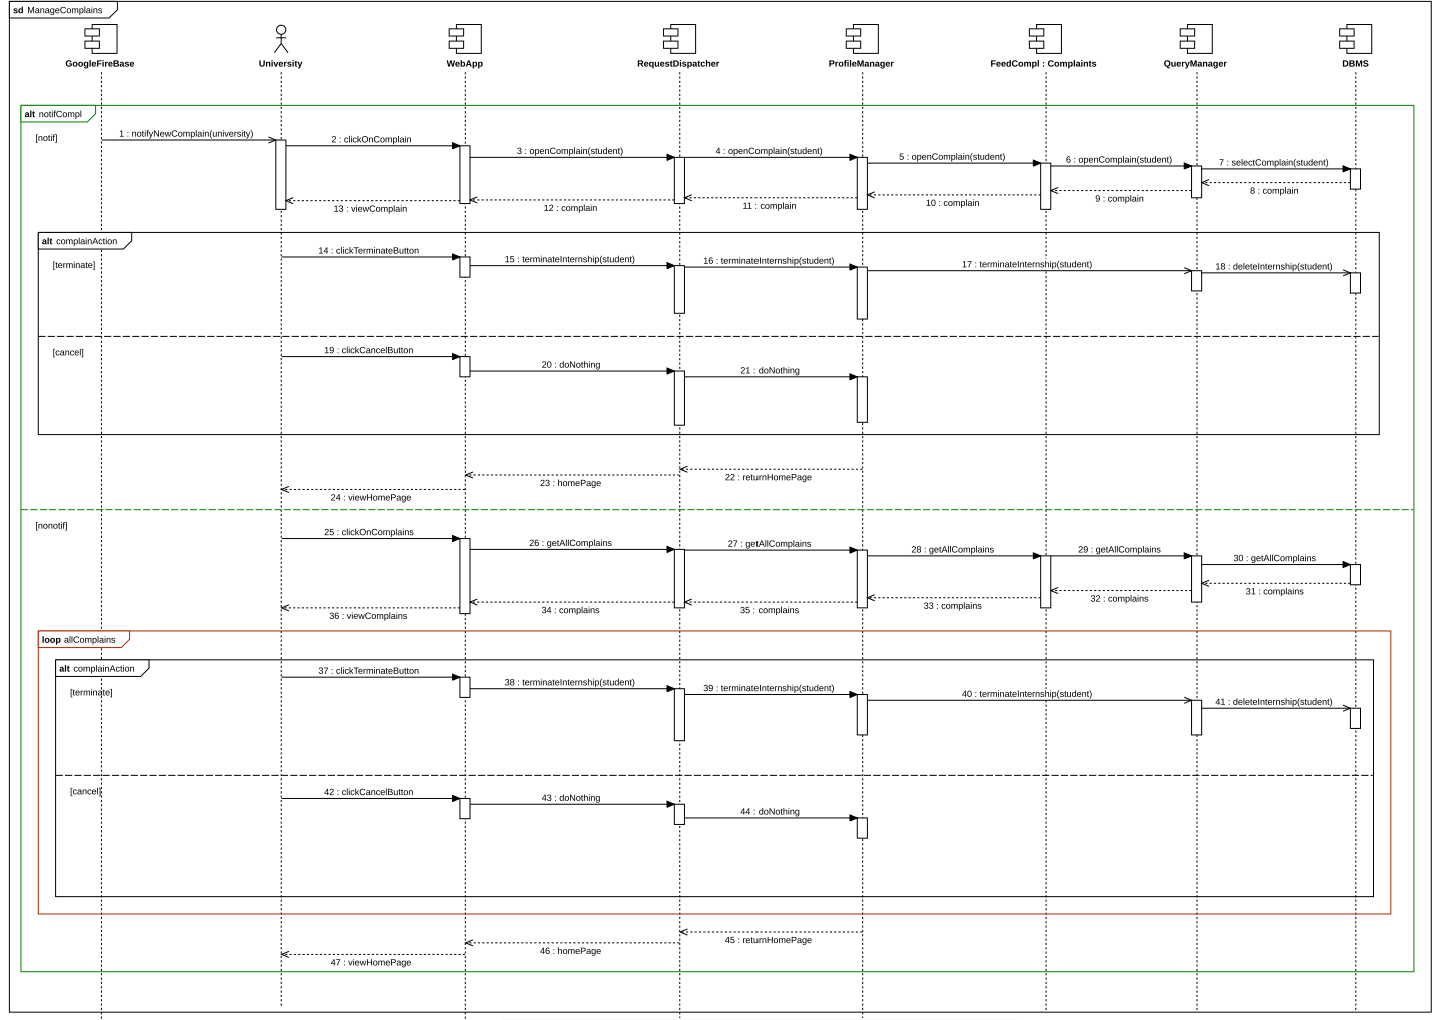
\includegraphics[width=1\linewidth]{SequenceDiagram/ManageComplSD.png}
    \caption{ManageComplains Sequence Diagram}
    \label{fig:enter-label}
\end{figure}
This sequence diagram allows the university to interact with the system to view complaints from its students regarding various internships. To do this, they either receive a notification from the system, or they manually open their homepage and then decide whether to close the internship or not.

\subsubsection{Internship publication}

\begin{figure}[H]
    \centering
    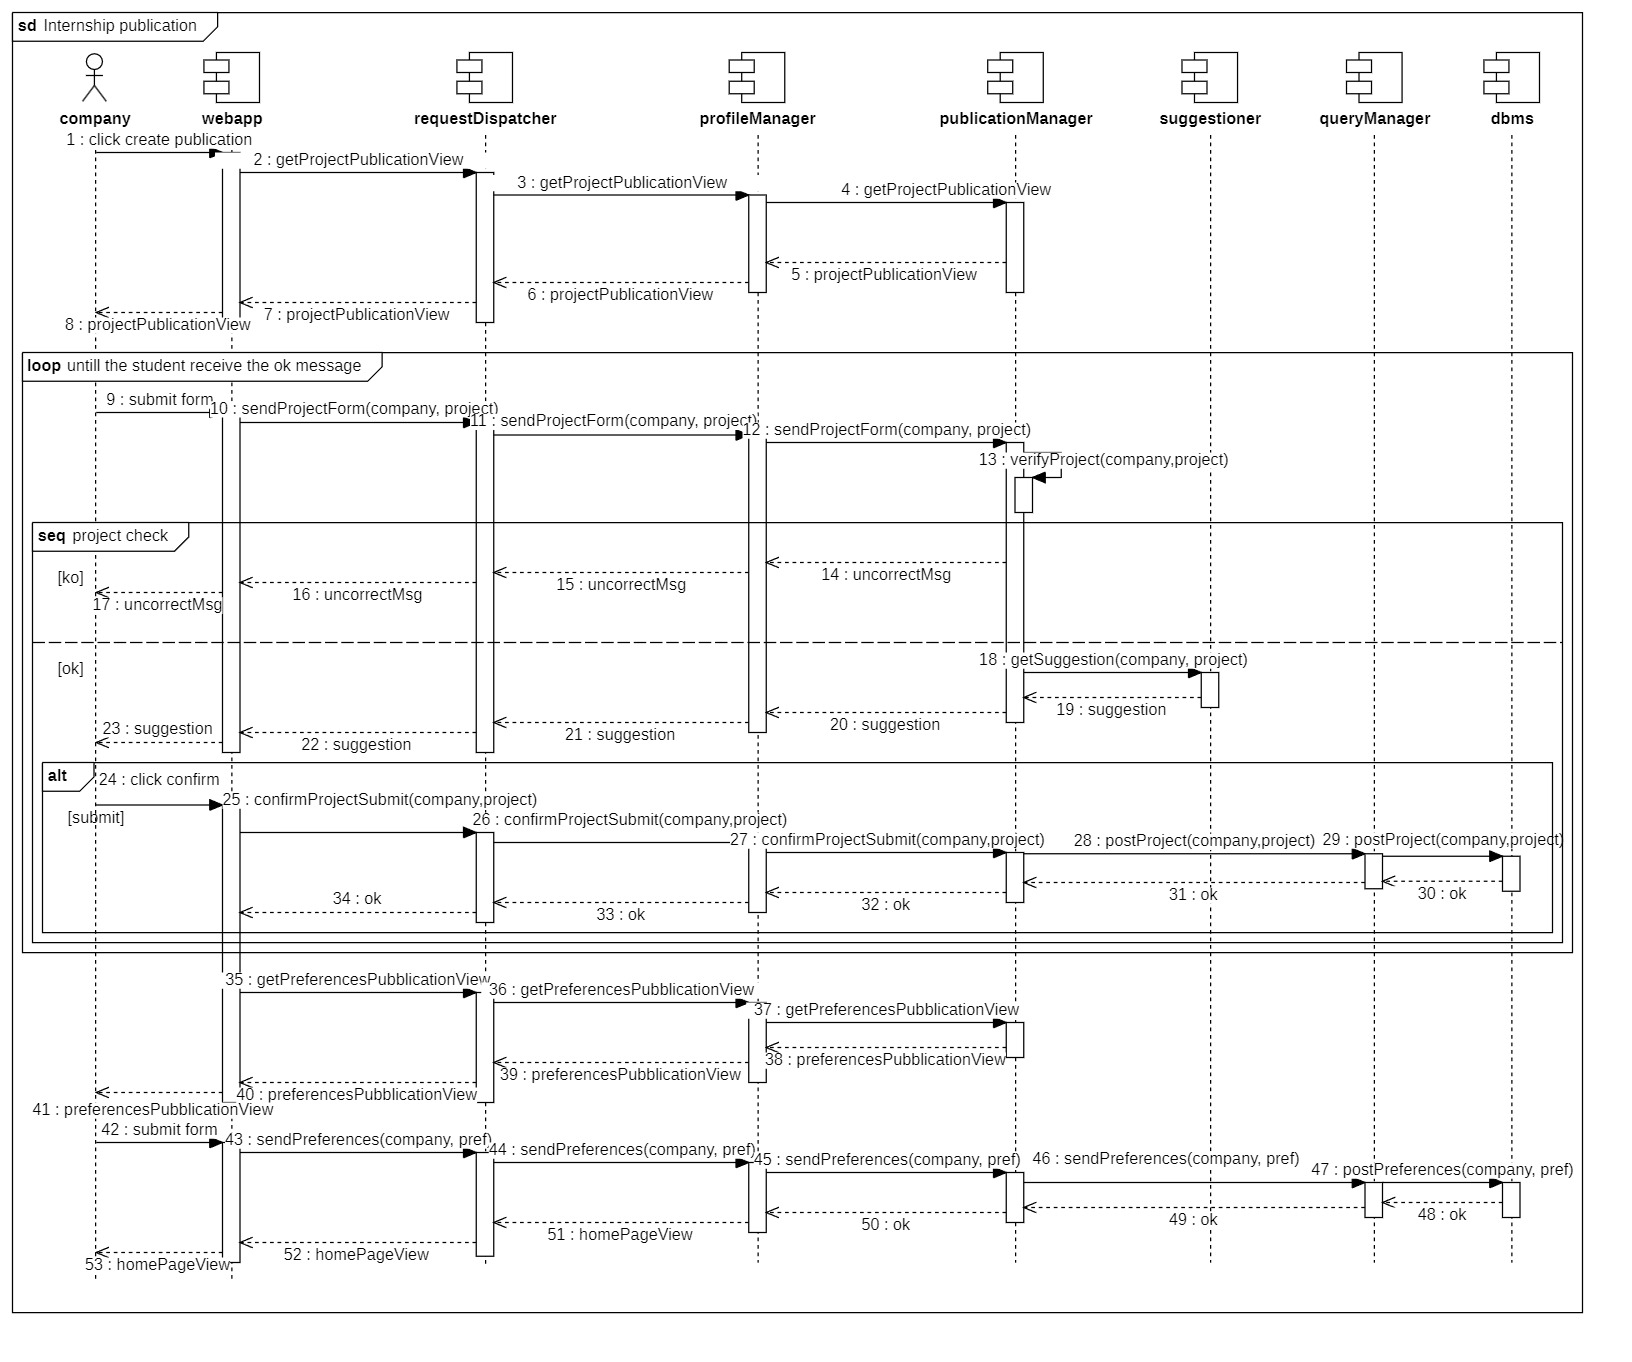
\includegraphics[width=1\linewidth]{SequenceDiagram/Internship publication.jpg}
    \caption{Internship publication diagram}
    \label{fig:enter-label}
\end{figure}
This sequence diagram allows the company to upload the project, with the possibility of using the software to obtain suggestions, and to publish the necessary requirements.

\subsubsection{ManagePublication company}
\begin{figure}[H]
    \centering
    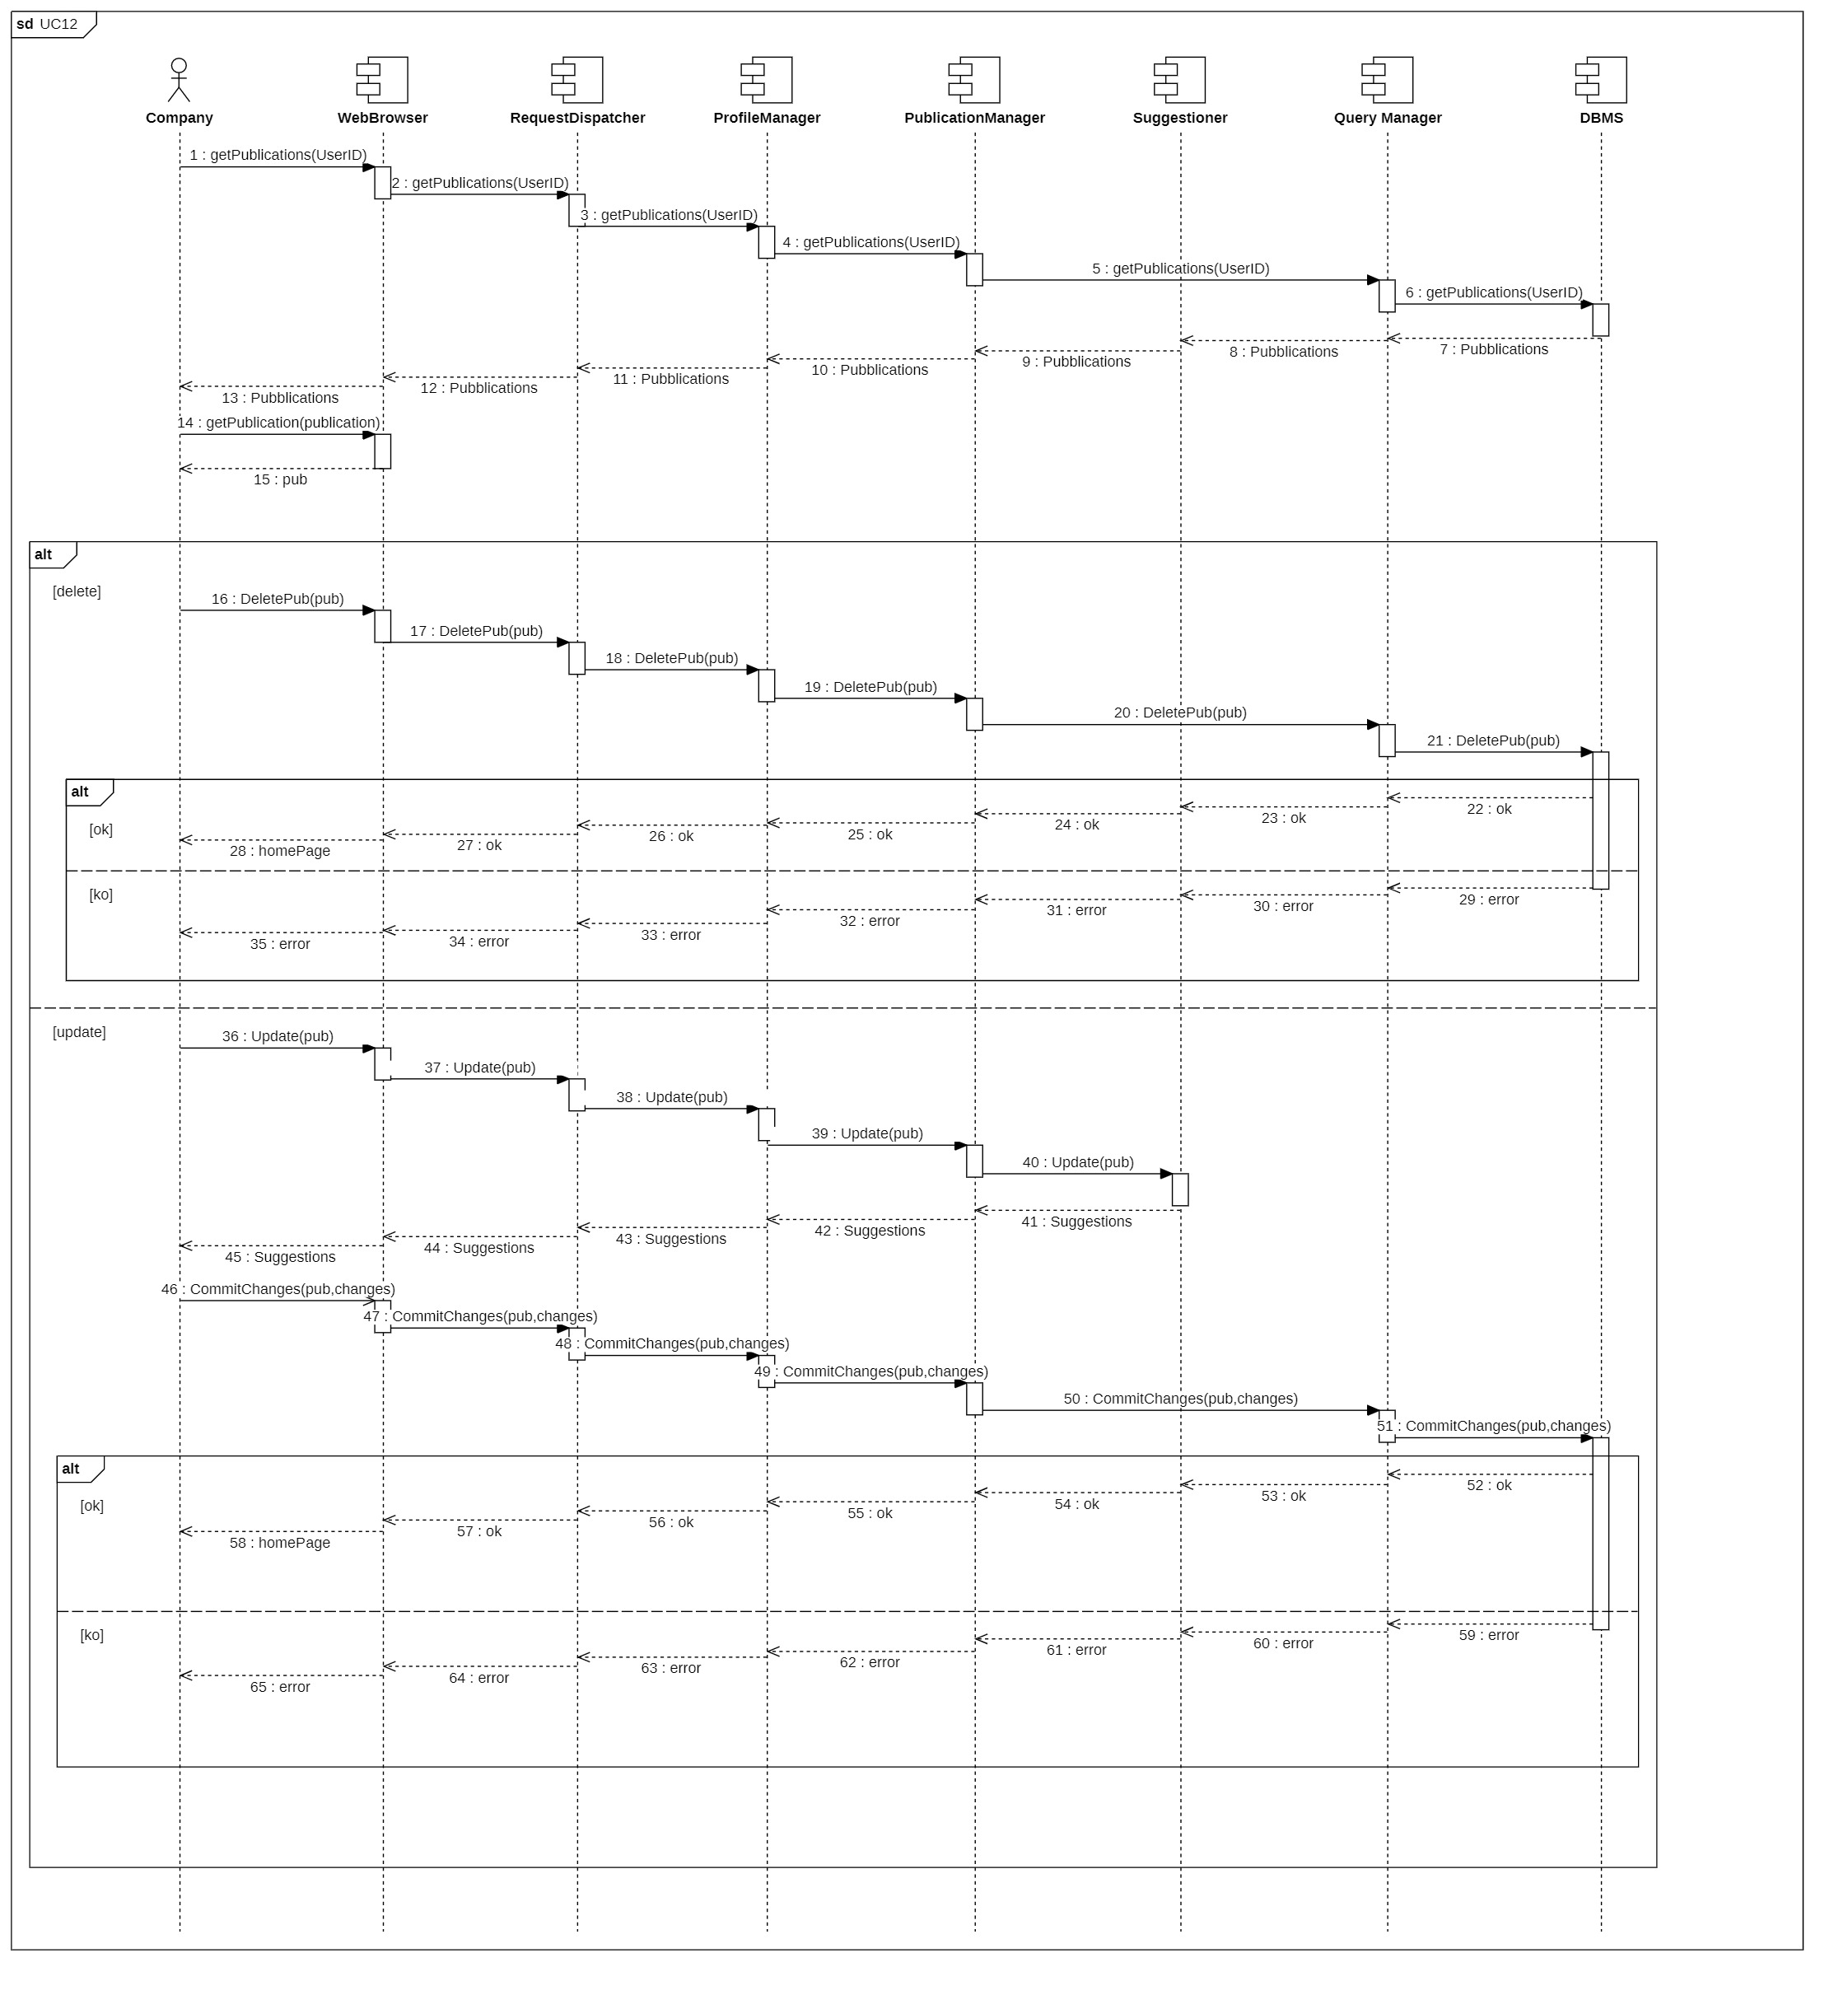
\includegraphics[width=1\linewidth]{SequenceDiagram/UC12.jpg}
    \caption{ManagePublication Sequence Diagram}
    \label{fig:enter-label}
\end{figure}
The above sequence diagram describes the process of updating an internship publication carried out by a company. After getting all its publications and selecting the wanted one, the company can choose whether to update or delete it. 

\subsubsection{AcceptDeclineMatch company}
\begin{figure}[H]
    \centering
    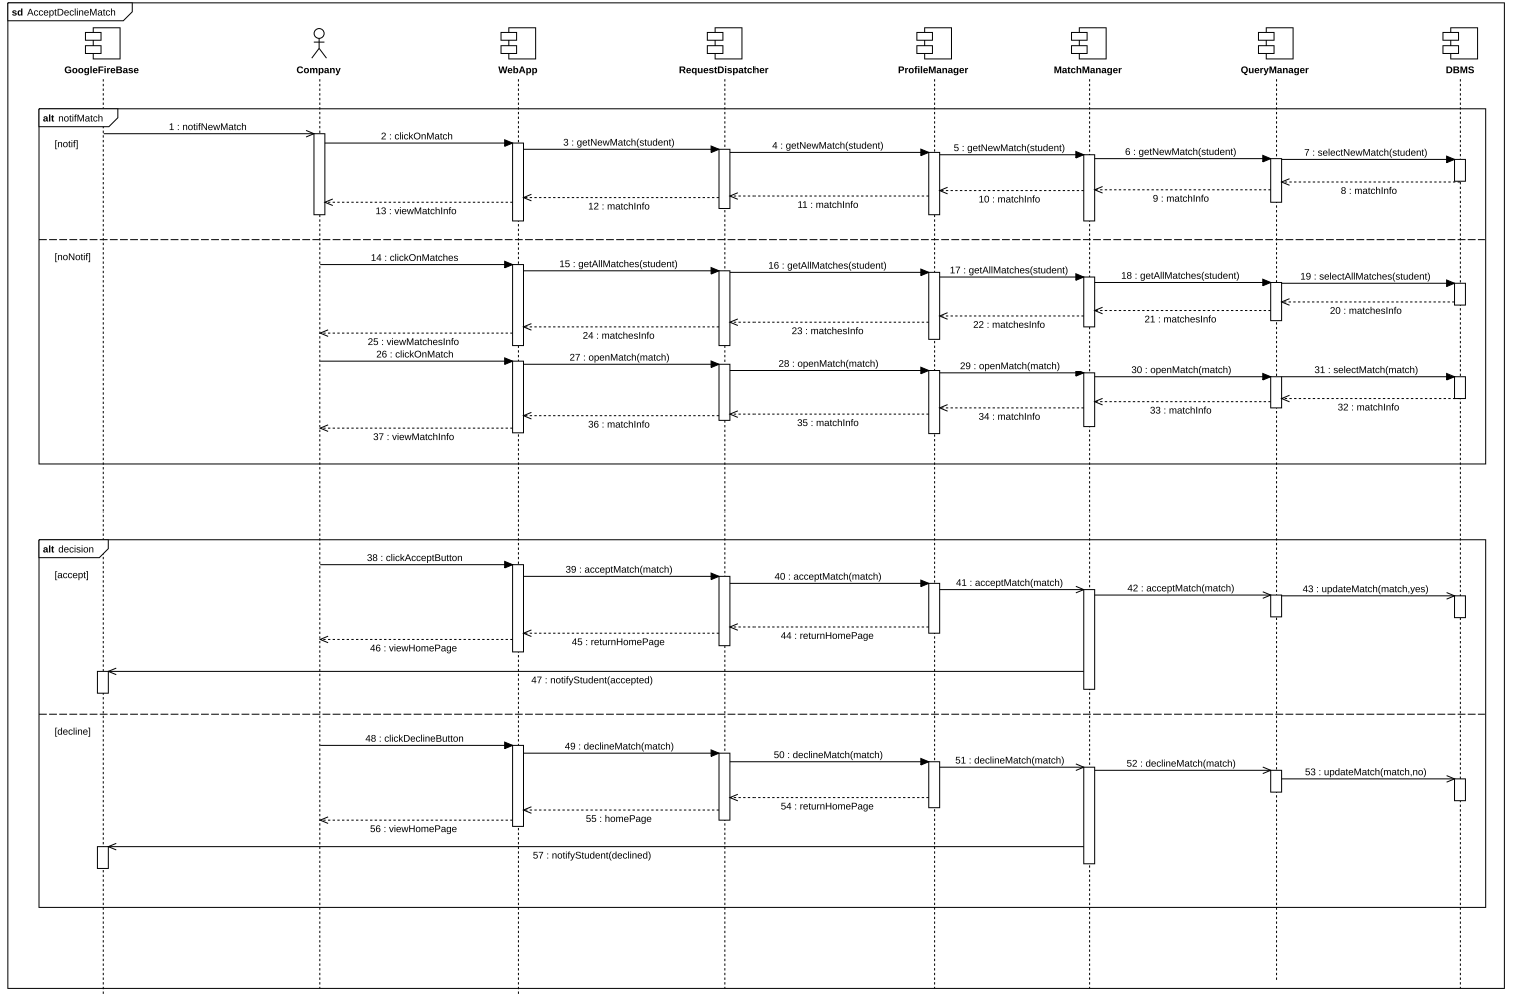
\includegraphics[width=1\linewidth]{SequenceDiagram/AccDeclMatchSD.png}
    \caption{AcceptDeclineMatch Sequence Diagram}
    \label{fig:enter-label}
\end{figure}
This sequence diagram allows the company to interact with the system to accept or reject a new match. To do this, they either receive a notification from the system, or they manually open the section with the found matches, and then decide whether to accept or reject the match. The system then notifies the corresponding student of the choice. 
\subsubsection{AcceptDeclineStudent}
\begin{figure}[H]
    \centering
    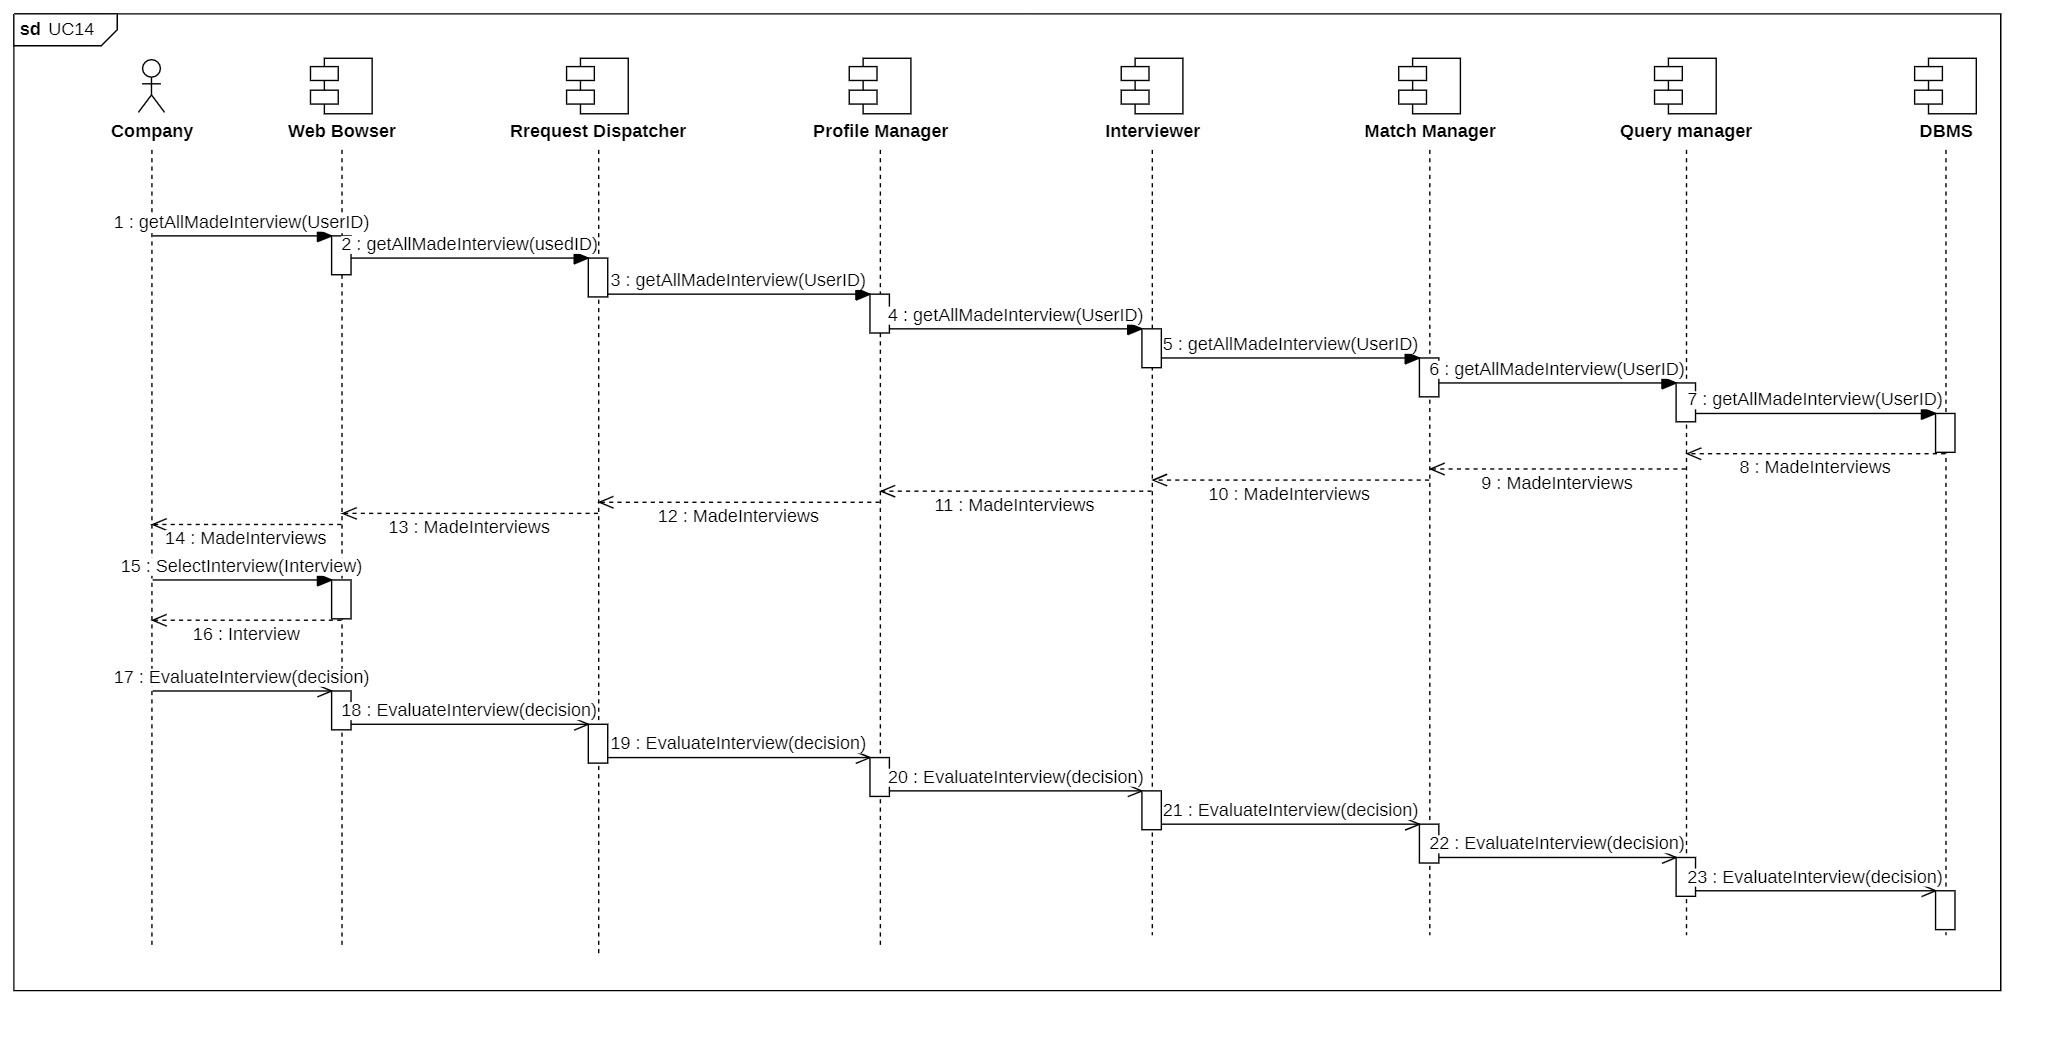
\includegraphics[width=1\linewidth]{SequenceDiagram/UC14.jpg}
    \caption{AcceptDeclineStudent  Sequence Diagram}
    \label{fig:enter-label}
\end{figure}
The sequence diagram in figure 19 shows how a company can accept or decline a student after the interview has been made. Once the wanted interview is selected, using the function EvaluateInterview, the decision (accepted/rejected) is passed as a parameter. The system will be then updated with that information and the user will eventually see the company decision 


\subsubsection{PublishComplaint company}
\begin{figure}[H]
    \centering
    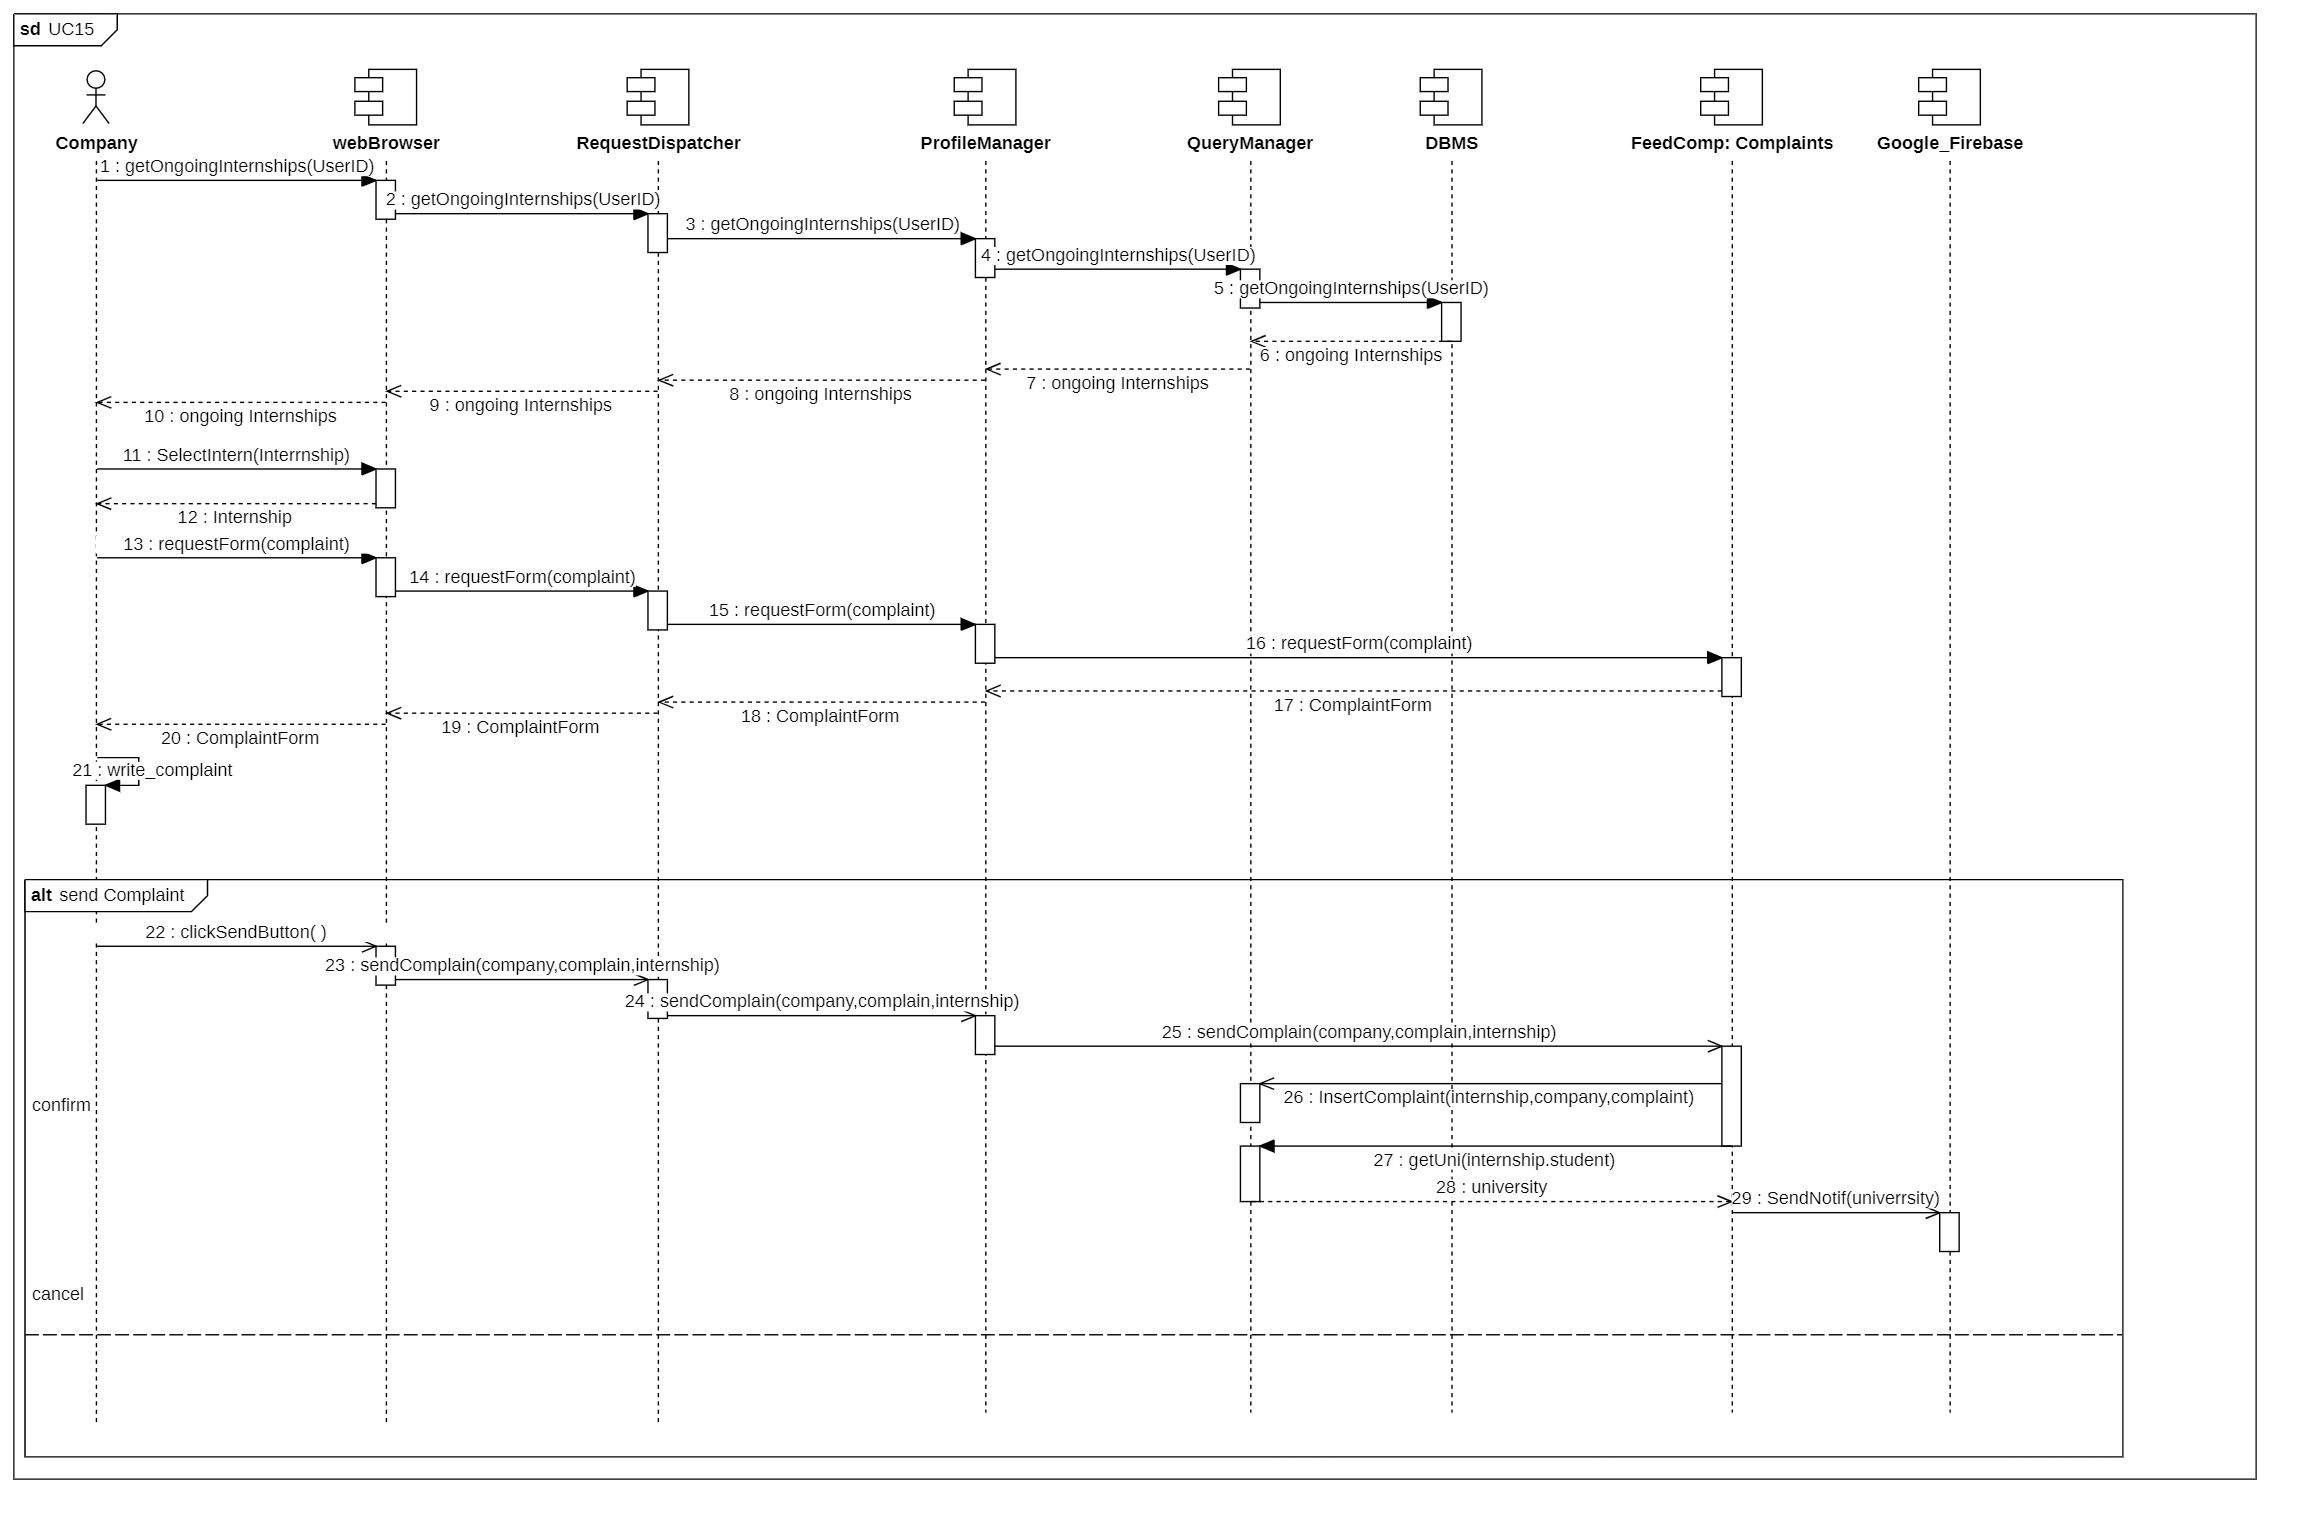
\includegraphics[width=1\linewidth]{SequenceDiagram/UC15.jpg}
    \caption{PublishComplaint  Sequence Diagram}
    \label{fig:enter-label}
\end{figure}
If a company has a complaint regarding an internship, it can select the needed one among all the others and start a complaint procedure (the function requestForm). Once the complaint is written, it's sent to the system which will upload it in the DB and send a notification to the university which will eventually take actions. 

\subsubsection{PublishFeedback company}
\begin{figure}[H]
    \centering
    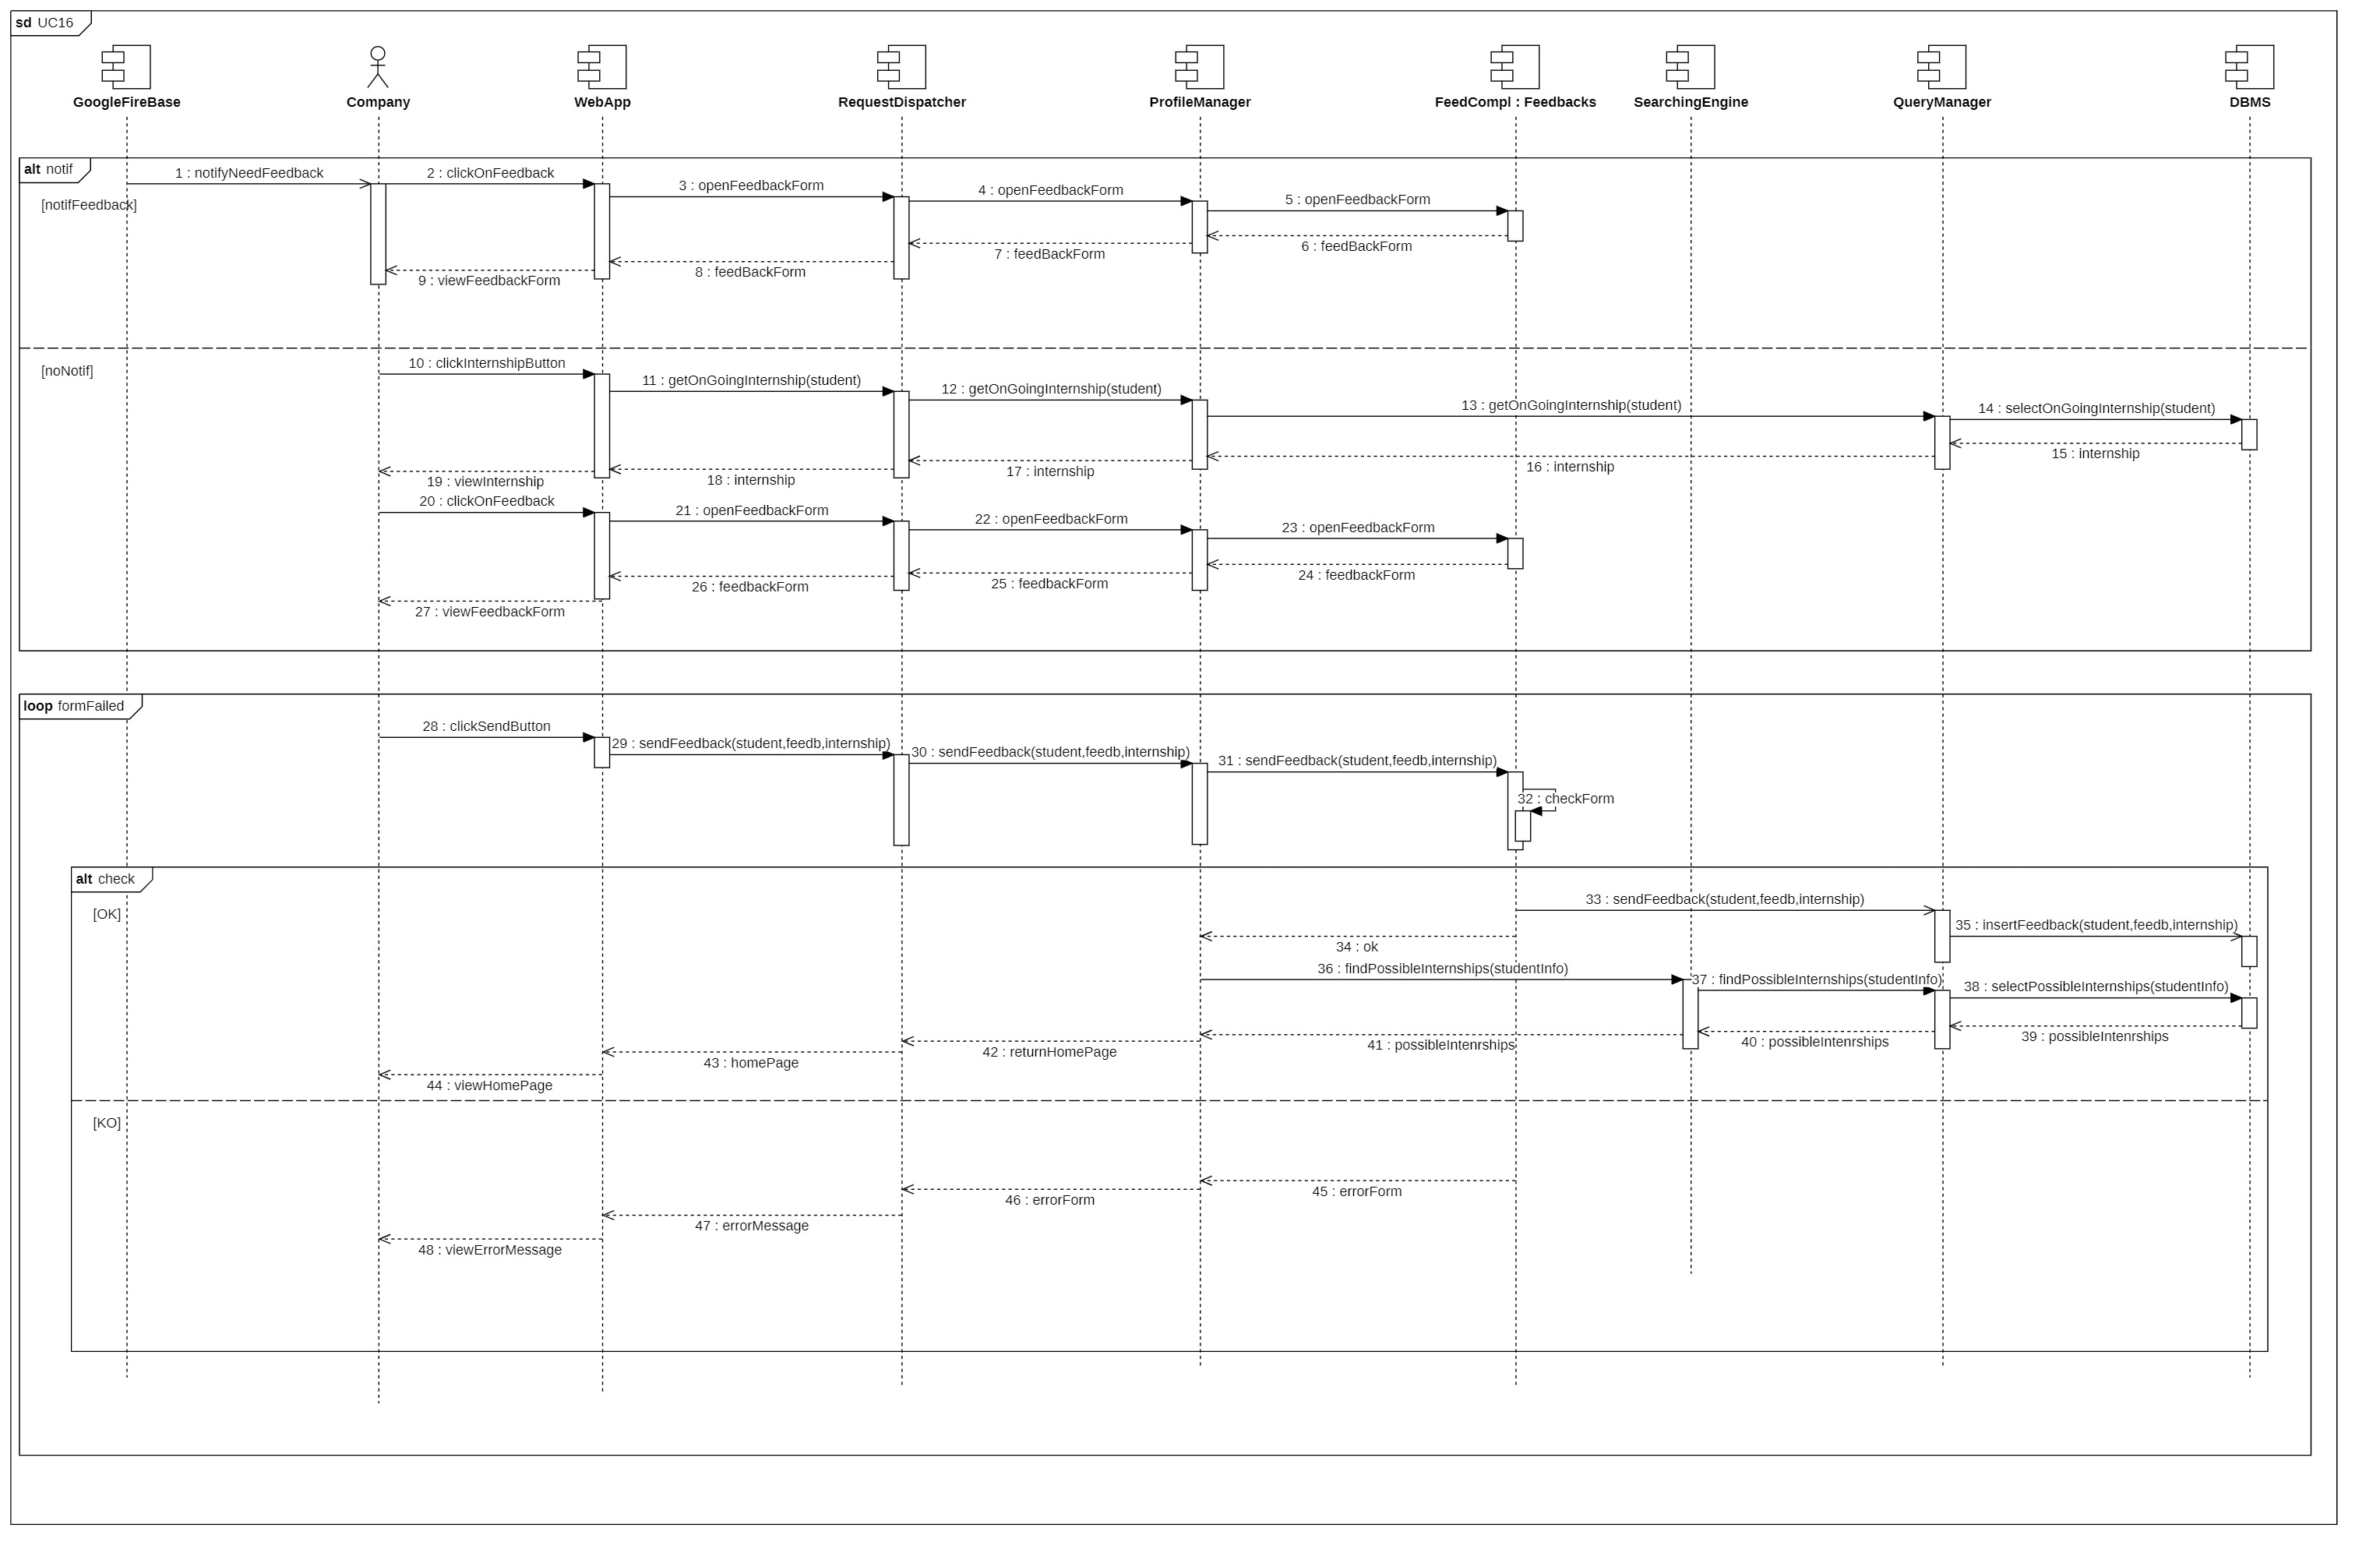
\includegraphics[width=1\linewidth]{SequenceDiagram/UC16.jpg}
    \caption{PublishFeedback  Sequence Diagram}
    \label{fig:enter-label}
\end{figure}
Once an internship is finished, the system will send a notification to both the user and the company, asking them to provide feedback about it. The "publishFeedback" procedure can begin by clicking the respective notification or by selecting the specific internship and calling the OpenFeedbackForm. Once the feedback is written, it is sent to the queryManager, which is in charge of uploading it to the DB. Simultaneously, the system uses the new information to update the internship suggestions.


\subsubsection{MakeInterviews}
\begin{figure}[H]
    \centering
    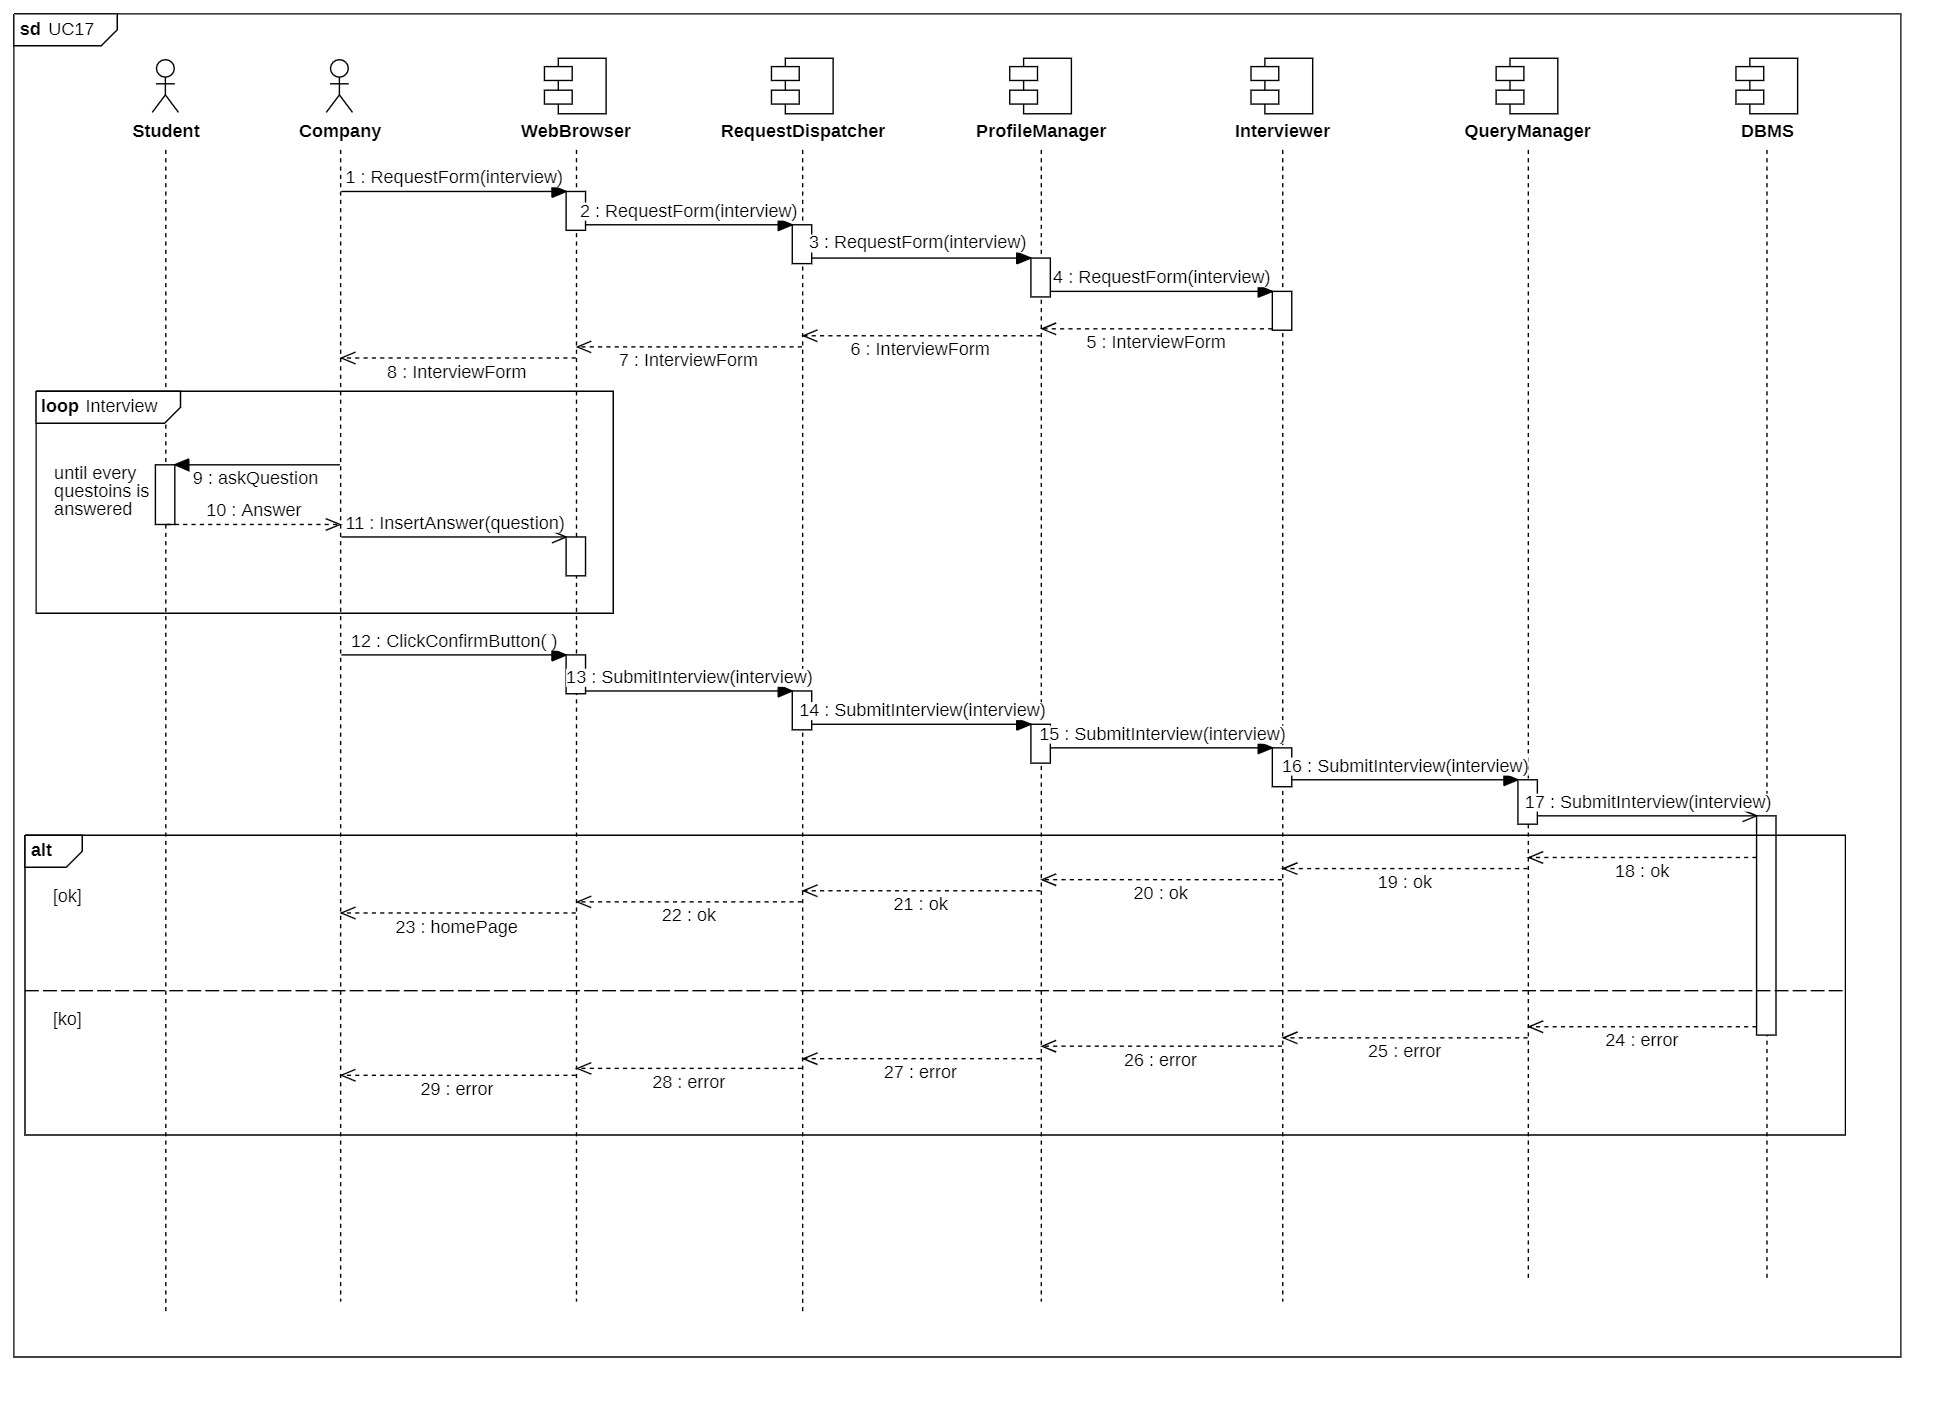
\includegraphics[width=1\linewidth]{SequenceDiagram/UC17.jpg}
    \caption{MakeInterviews  Sequence Diagram}
    \label{fig:enter-label}
\end{figure}
The interview process is described in the above diagram. Once the company has generated the interview form, it asks the form's questions to the user and fills out the form with the student's answers. Once the form is complete, it is sent to the query manager, which will save it to the DB.
    
\subsubsection{Match making}

\begin{figure}[H]
    \centering
    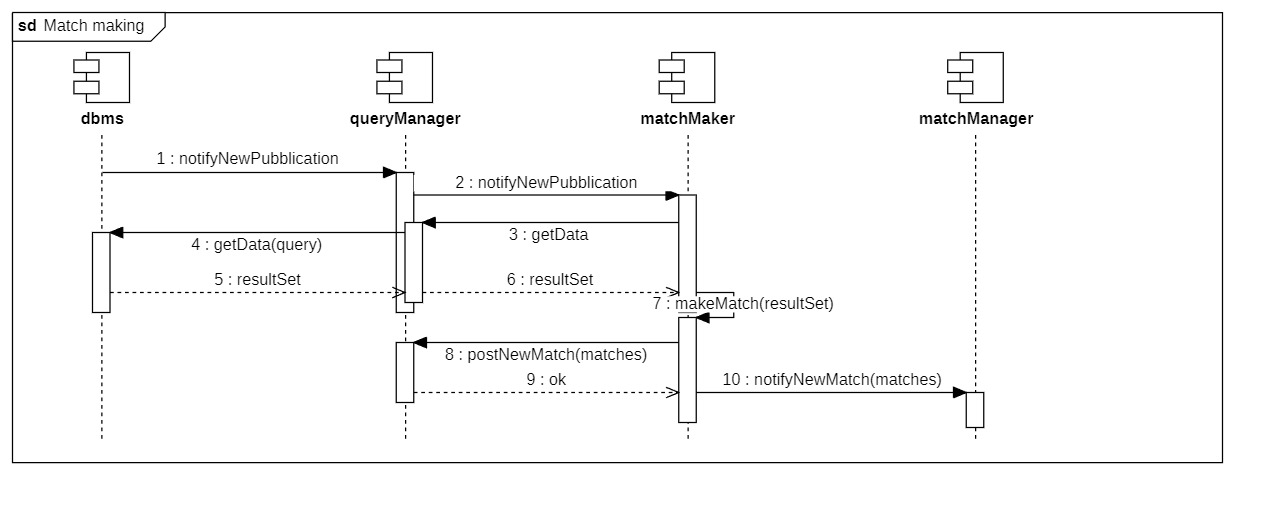
\includegraphics[width=1\linewidth]{SequenceDiagram/Match making.jpg}
    \caption{Match making Sequence diagram}
    \label{fig:enter-label}
\end{figure}
This component is responsible for initiating matchmaking after a publication is inserted or modified in the database.
\subsection{Component Interfaces}

\subsubsection{RequestDispatcher}
\begin{enumerate}
    \item sendFormLogin(email,psw)
    \item getNewMatch(student)
    \item getAllMatches(student)
    \item openMatch(match)
    \item acceptMatch(match)
    \item declineMatch(match)
    \item getOnGoingInternship(student)
    \item openComplainForm()
    \item sendComplain(user,complain,internship)
    \item openComplain(student)
    \item getAllComplains()
    \item terminateInternship(student)
    \item doNothing()
    \item goToHomePage()
    \item openFeedbackForm()
    \item sendFeedback(student,feedb,internship)
    \item getPublicationView()
    \item getPublication(UserID)
    \item sendCvForm(student,cv)
    \item confirmCvSubmit(student,cv)
    \item getPreferencesPublicationView()
    \item sendPreferences(company, pref)
    \item getCvModificationView(student)
    \item deleteCv(student)
    \item sendUpdateCv(student,cv)
    \item sendChanges(student,changes)
    \item getProjectPublicationView()
    \item sendProjectForm(company, project)
    \item getCompanyPage(company)
    \item sendApplicationRequest(student,company)
    \item getPublilcationModificationView()
    \item deletePub(pub)
    \item signUp(data)
    \item update(pub)
    \item commitChanges(pub,changes)
    \item getAllMadeInterview(userID)
    \item evaluate(interview)
    \item getOngoingInternships(userID)
    \item requestForm(formType)
    \item SubmitInterview(interview)
    \item DeletePub(pub)
    \item Update(pub)
    \item EvaluateInterview(decision)
    \item getOngoingInternships(UserID)
    \item confirmCvUpdate(student, cv)
    \item confirmProjectSubmit(company,project)
    \item getCvPubblicationView()
\end{enumerate}

\subsubsection{Auth:Registrator}
\begin{enumerate}
    \item SignUP(data)
\end{enumerate}

\subsubsection{Auth:Authenticator}
\begin{enumerate}
    \item sendFormLogin(email,psw)
\end{enumerate}

\subsubsection{Searching Engine}
\begin{enumerate}
    \item findPossibleInternships(student)
    \item getCompanyPage(company)
\end{enumerate}

\subsubsection{Profile Manager}
\begin{enumerate}
    \item findPossibleInternships(student)
    \item getNewMatch(student)
    \item getAllMatches(student)
    \item openMatch(match)
    \item acceptMatch(match)
    \item declineMatch(match)
    \item getOnGoingInternship(student)
    \item terminateInternship(student)
    \item doNothing()
    \item openComplainForm()
    \item sendComplain(user,complain,internship)
    \item openComplain(student)
    \item getAllComplains()
    \item openFeedbackForm()
    \item sendFeedback(student,feedb,internship)
    \item goToHomePage()
    \item getPublicationView()
    \item sendCvForm(student,cv)
    \item confirmCvSubmit(student,cv)
    \item getPreferencesPublicationView()
    \item sendPreferences(company, pref)
    \item getCvModificationView(student)
    \item deleteCv(student)
    \item sendUpdateCv(student,cv)
    \item sendChanges(student,changes)
    \item getProjectPublicationView()
    \item sendProjectForm(company, project)
    \item getPublilcationModificationView()
    \item deletePublication(student)
    \item getPublications(UserID)
    \item DeletePub(pub)
    \item Update(pub)
    \item CommitChanges(pub,changes)
    \item getAllMadeInterview(UserID)
    \item EvaluateInterview(decision)
    \item getOngoingInternships(UserID)
    \item requestForm(formType)
    \item submitInterview(interview)
    \item confirmCvUpdate(student, cv)
    \item confirmProjectSubmit(company,project)
    \item getCvPubblicationView()
\end{enumerate}

\subsubsection{Publication Manager}
\begin{enumerate}
    \item getPublicationView()
    \item sendCvForm(student,cv)
    \item confirmCvSubmit(student,cv)
    \item getPreferencesPublicationView()
    \item sendPreferences(company, pref)
    \item checkCV(student, cv) 
    \item getCvModificationView(student)
    \item deleteCv(student)
    \item sendUpdateCv(student,cv)
    \item sendChanges(student,changes)
    \item verifyChanges(student, changes)
    \item getProjectPublicationView()
    \item sendProjectForm(company, project)
    \item verifyProject(company,project)
    \item getPublilcationModificationView()
    \item deletePublication(student)
    \item getPublications(UserID)
    \item DeletePub(pub)
    \item Update(pub)
    \item CommitChanges(pub,changes)
    \item confirmCvUpdate(student, cv)
    \item confirmProjectSubmit(company,project)
    \item getCvPubblicationView()
\end{enumerate}

\subsubsection{Suggestioner}
\begin{enumerate}
    \item getSuggestion(student,cv)
    \item getSuggestion(company, project)
    \item Update(pub)
\end{enumerate}

\subsubsection{MatchMaker}
\begin{enumerate}
    \item notifyNewPubblication()
    \item makeMatch(resultSet)
\end{enumerate}

\subsubsection{MatchManager}
\begin{enumerate}
    \item getNewMatch(student)
    \item getAllMatches(student)
    \item openMatch(match)
    \item acceptMatch(match)
    \item declineMatch(match)
    \item add\&notifyMatch(student, company)
    \item notifyNewMatch(matches)
    \item getAllMadeInterview(UserID)
    \item evaluateInterview(decision)
\end{enumerate}

\subsubsection{QueryManager}
\begin{enumerate}
    \item sendFormLogin(email,psw)
    \item findPossibleInternships(student)
    \item getNewMatch(student)
    \item getAllMatches(student)
    \item openMatch(match)
    \item acceptMatch(match)
    \item declineMatch(match)
    \item getOnGoingInternship(student)
    \item terminateInternship(student)
    \item sendComplain(student,complain,internship)
    \item sendFeedback(student,feedb,internship)
    \item openComplain(student)
    \item getAllComplains()
    \item postCv(cv)
    \item postPreference(preference)
    \item deleteCv(student)
    \item postProject(company,project)
    \item getCompanyPage(company)
    \item deletePublication(student)
    \item notifyNewPubblication()
    \item getData()
    \item postNewMatch(matche)
    \item signUP(data)
    \item registerNewUser(data)
    \item getPublications(UserID)
    \item DeletePub(pub)
    \item CommitChanges(pub,changes)
    \item getAllMadeInterview(UserID)
    \item EvaluateInterview(decision)
    \item getOngoingInternships(UserID)
    \item InsertComplaint(internship,company,complaint)
    \item getUni(internship.student)
    \item submitInterview(interview)
    \item postChanges(student,changes)
\end{enumerate}

\subsubsection{Feedbacks\_Complaints:Feedbacks}
\begin{enumerate}
    \item openFeedbackForm()
    \item sendFeedback(student,feedb,internship)
\end{enumerate}

\subsubsection{Feedbacks\_Complaints:Complaints}
\begin{enumerate}
    \item openComplainForm()
    \item sendComplain(user,complain,internship)
    \item openComplain(student)
    \item getAllComplains()
    \item requestForm(formType)
\end{enumerate}

\subsubsection{Interviewer}
\begin{enumerate}
    \item getAllMadeInterview(UserID)
    \item evaluatInterview(decision)
    \item createInterviewForm()
    \item requestForm(formType)
    \item submitInterview(interview)
\end{enumerate}


\subsection{Selected architectural styles and patterns}
\subsubsection{3-tier Architecture}
We decided to use a 3-tier architecture because:
\begin{enumerate} 
    \item it facilitates the separation of the system into independent layers (such as presentation, business logic, and data access) and tiers (including client, application server, and DBMS), making the system more modular and simpler to update or manage. 
    \item the distinction between layers and tiers simplifies scaling the system by allowing the distribution of workloads across several servers. 
    \item the architecture supports the implementation of load balancing and caching methods to enhance performance.
\end{enumerate}

\subsubsection{Client-Server Architecture}
The system's behavior will primarily follow a Client-Server architecture, where the Client acts as the front-end user interface while the Server functions as the back-end platform, processing user requests, performing computations, and providing responses.\newline
In a traditional Client-Server architecture, the Client always initiates the requests, while the Server remains a passive entity that processes these requests and returns the corresponding responses. However, in certain scenarios, such as interacting with the Google Firebase component to send notifications, the Server must execute actions without being prompted by the Client, making it an active component with a more Event-Driven approach.

\subsubsection{REST API}
We decided to implement a REST API to simplify communication between the client and server, as it provides numerous advantages. The API leverages standard web technologies (HTTPS), making it straightforward to use and integrate with other systems. Its stateless nature ensures that each request operates independently of others. Furthermore, using a REST API enhances scalability, as the separation between Client and Server allows for independent modifications or updates to each component.

\subsubsection{Model-View-Controller pattern}
The implementation of S\&C will adopt the Model-View-Controller pattern, a software design approach that divides the software into three interconnected components:
\begin{itemize} 
    \item \textbf{Model}: includes the methods responsible for data management. It provides functionality for saving, retrieving, and modifying data in the database.    
    \item \textbf{View}: focuses on the visual presentation of data to the end user.
    \item \textbf{Controller}: serves as the intermediary between the view and the model. It manages user interactions with the view and processes the corresponding operations.
\end{itemize}

\subsection{Other Design Decisions}
\subsubsection{Availability}
The incorporation of load balancing and replication mechanisms greatly improves the reliability and availability of our system. Load balancing maximizes resource efficiency by evenly distributing incoming requests among servers, thereby avoiding performance bottlenecks. At the same time, replication enhances fault tolerance by duplicating critical services. This redundancy reduces the effects of potential failures, ensuring that our system can sustain service availability even under adverse conditions.

\subsubsection{Scalability}
The Service-Oriented Architecture (SOA) promote scalability through several key principles. SOA structures an application as a collection of services, which can be independently deployed and managed. This modularity allows for selective scaling of individual services based on demand. For instance, if a specific service, such as order processing, experiences a surge in traffic, only that service needs to be scaled up, rather than the entire application.

\subsubsection{Notification Handling}
To send notifications to users of the app, we use an external tool called "GoogleFireBase". This tool allows us to send push messages directly to users when needed, without the app having to manage everything internally. For example, we can notify users about new match created or new complains. By integrating with GoogleFireBase, the process becomes much simpler and more efficient, enabling us to send targeted notifications quickly without building a complex solution from scratch.

\subsubsection{Relational Database}
We chose a relational database for our system design because it excels at storing structured data, maintaining data integrity, and delivering fast query performance. It is also scalable, capable of handling large volumes of data and supporting many simultaneous users. The database enables us to store and retrieve information efficiently, while ensuring that the data remains accurate and consistent.

\subsubsection{Ease of Deployment}
Adopting a SOA architecture offers a significant advantage in deployment ease. This approach allows changes to be made to individual services independently, enabling smooth deployments without affecting the entire system. This flexibility in deployment not only speeds up updates but also improves the system's resilience and agility, making troubleshooting and maintenance much more efficient.

\section{User Interface Design} 
\subsection{Overview}
\begin{figure}[H]
    \centering
    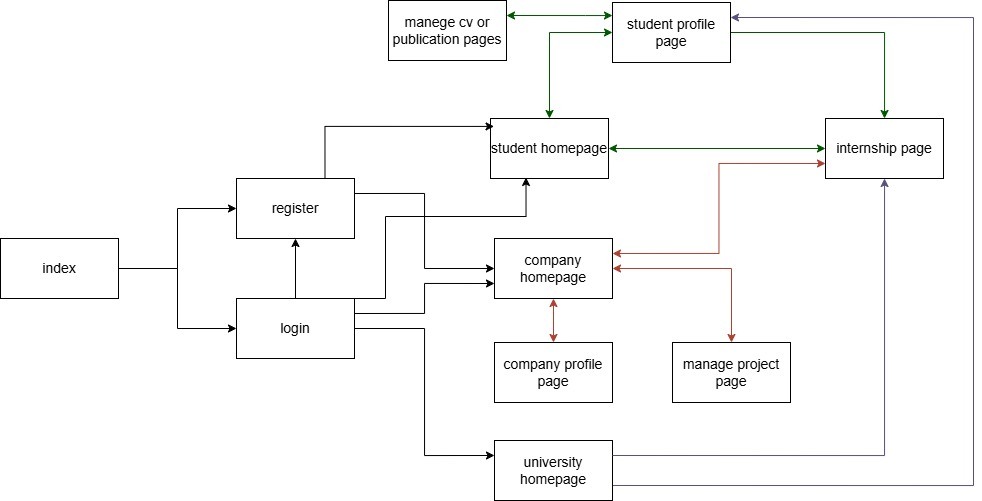
\includegraphics[width=1\linewidth]{interface/overviewInterface.jpg}
    \caption{overview of the user interface}
     \label{fig:overviewInterface}
\end{figure}
The figure \ref{fig:overviewInterface} show how a user, with the correct rights, can navigate through the pages. The rights are showd by usign differents color, green for the student, red for the companies and then purple for the university.

\subsection{Mockups}
In this section there are the most important pages that show how the user interfaces will be.
\begin{figure}[H]
    \centering
    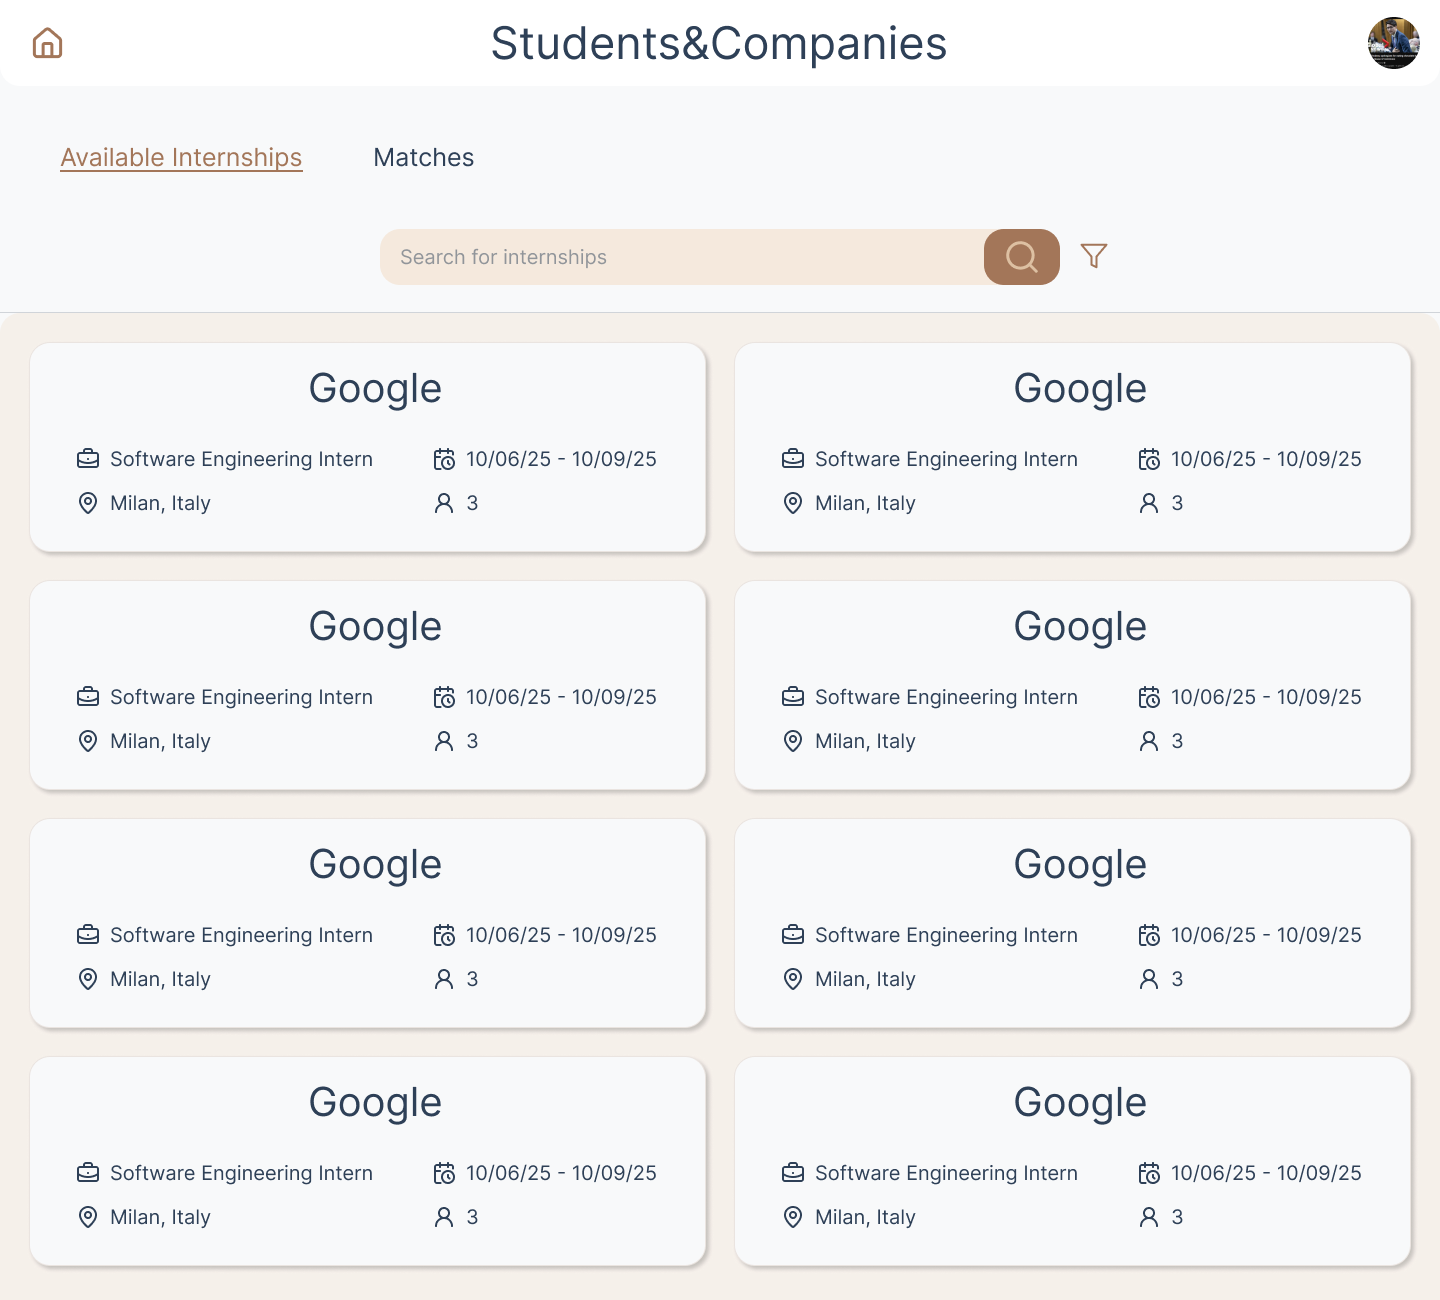
\includegraphics[width=1\linewidth]{interface/HomePage-studente- def.png}
    \caption{Student home page available internships}
    \label{fig:enter-label}
\end{figure}
This page shows all available internships, not just those found through matches, but any internship published by companies. The student can also search a particular internship, for example if he is looking for a specific company. Clicking on his profile image, he can go through it's profile page, while clicking on one internship he can go through the internship page.

\begin{figure}[H]
    \centering
    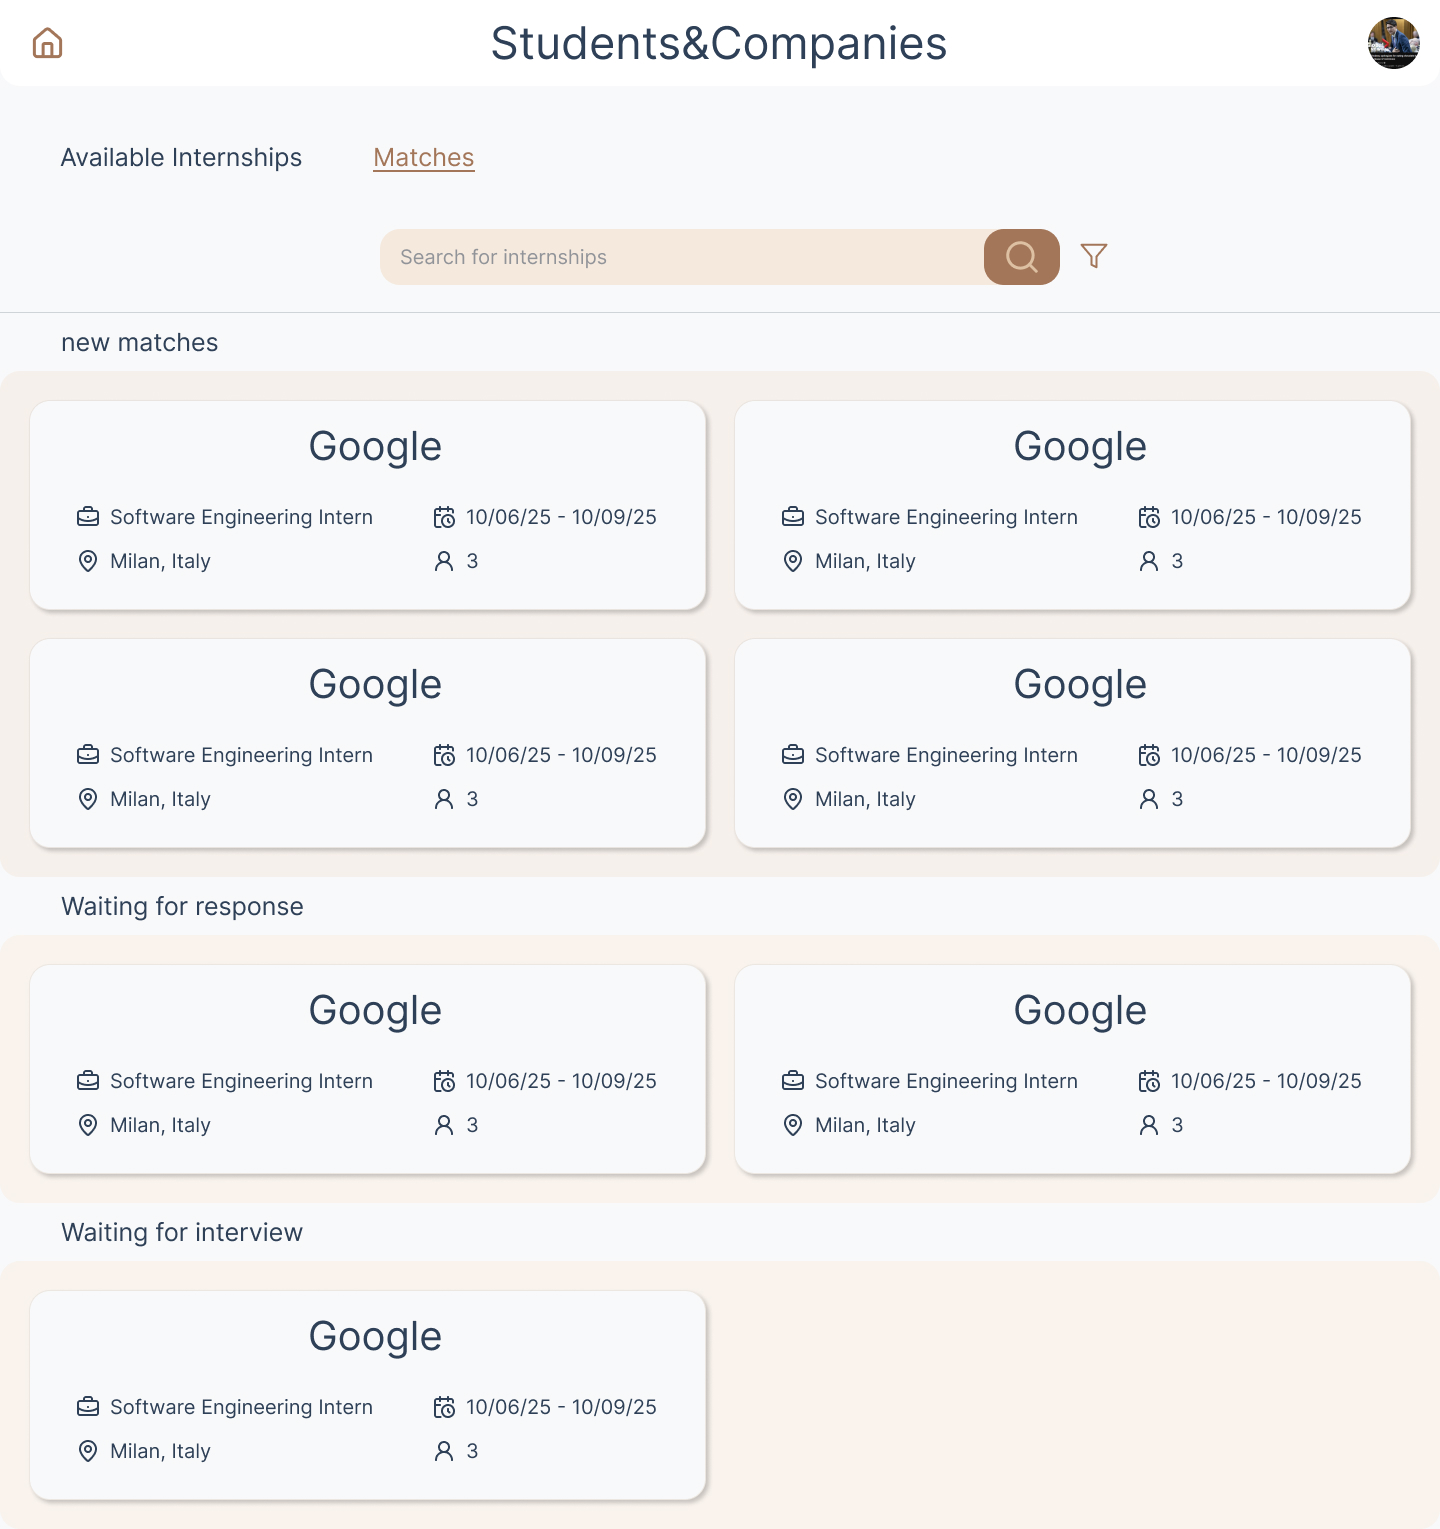
\includegraphics[width=1\linewidth]{interface/Match - Studente.jpg}
    \caption{Student home page match sections}
    \label{fig:enter-label}
\end{figure}
This page shows all available matches. The student can also search a particular internship, for example if he is looking for a specific company. Clicking on his profile image, he can go through it's profile page, while clicking on one internship he can go through the internship page.\newline
The 'new matches' show all the matches found and not accepted by anyone yet. The 'Waiting for response' show all the matches accepted by the student but not accepted by the company yet.
The 'Waiting for interview' show the match accepted by the company and by the student, but the company is making the interview and can still accept or decline the student.

\begin{figure}[H]
    \centering
    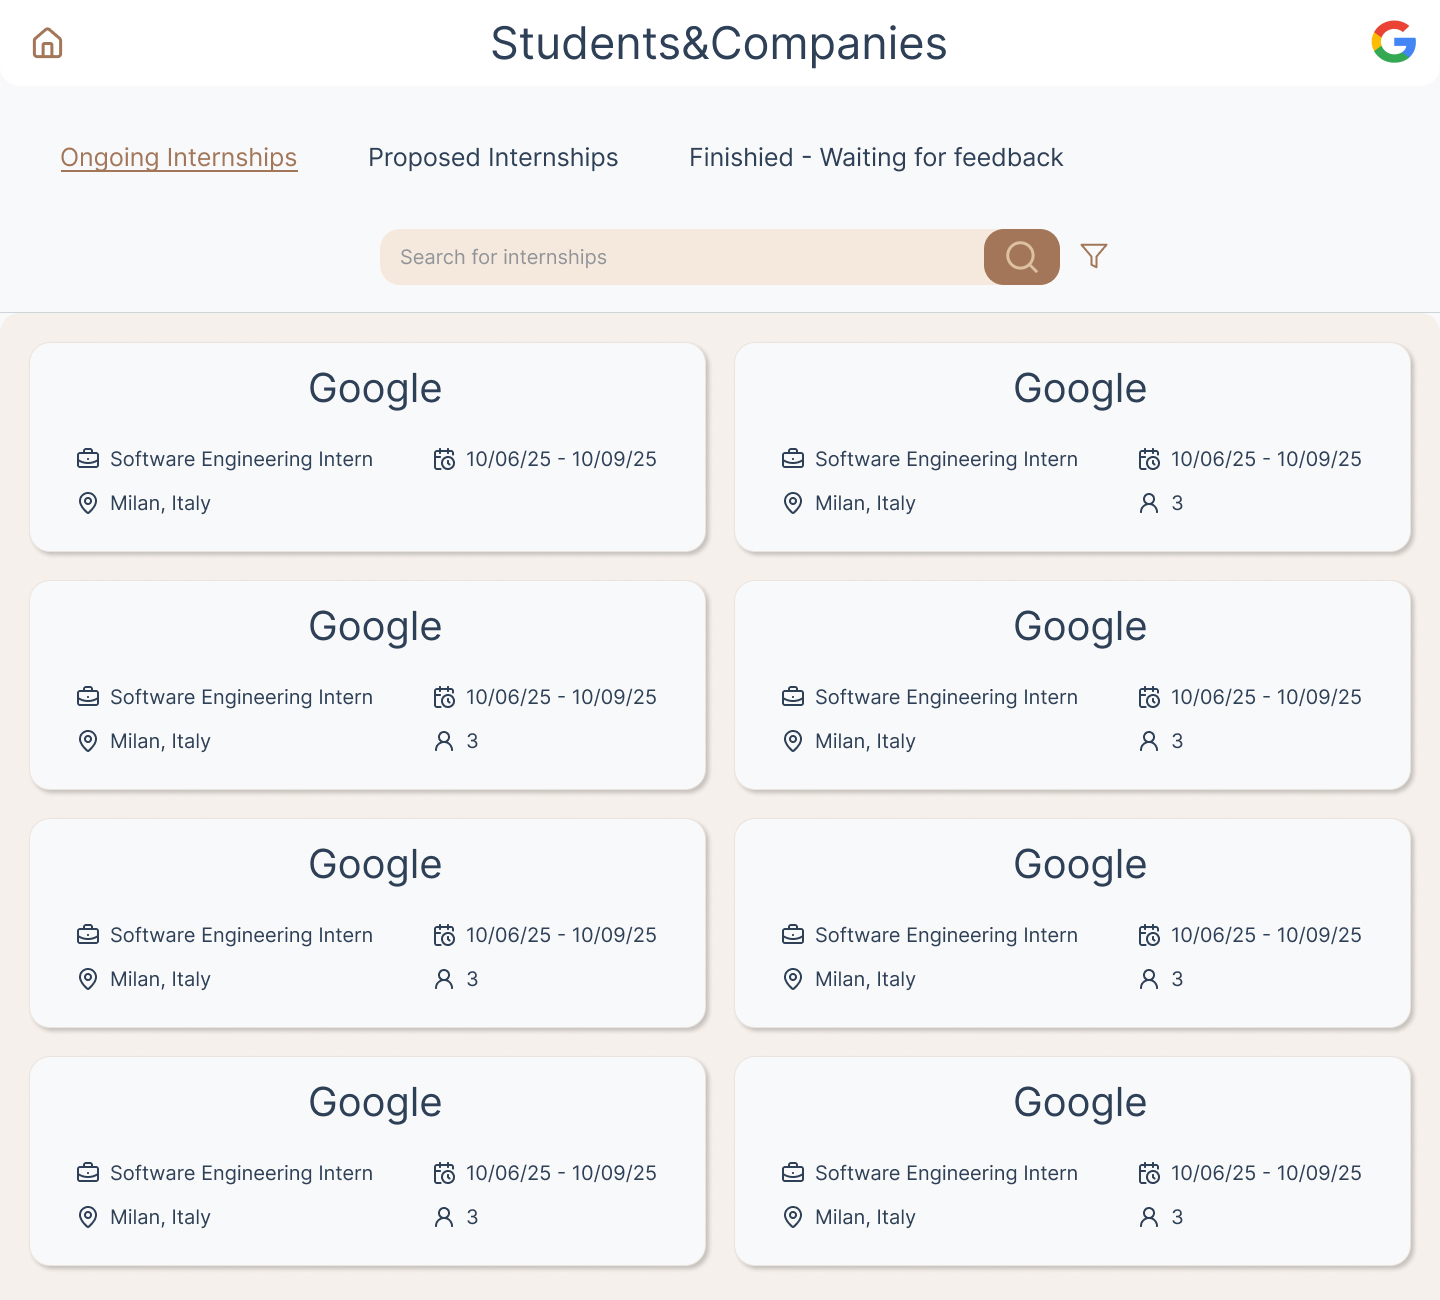
\includegraphics[width=1\linewidth]{interface/HomePage-Company.jpg}
    \caption{Company home page ongoing internships}
    \label{fig:enter-label}
\end{figure}
This page shows all the ongoing internships. Clicking on an internship the company will see the page with all the information about that ongoing internship. It can also goes to the 'Proposed Internships' and 'Finished - Waiting for feedback' sections. 

\begin{figure}[H]
    \centering
    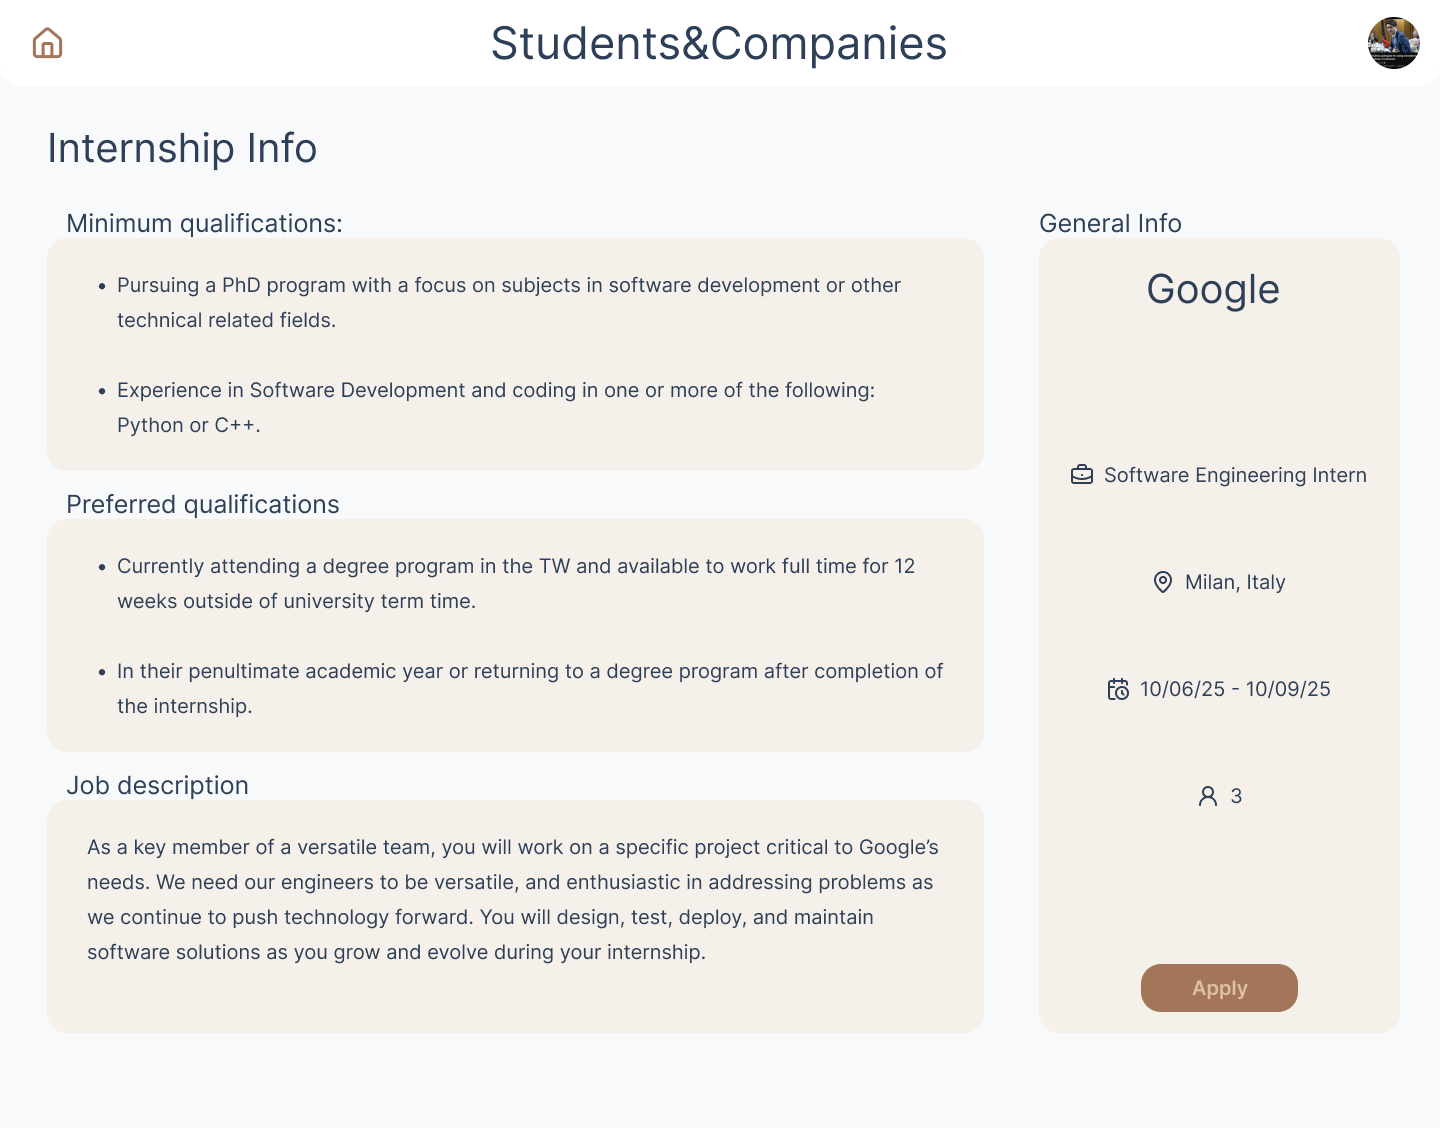
\includegraphics[width=1\linewidth]{interface/Internship view - Student.png}
    \caption{Internship view seen by a student}
    \label{fig:enter-label}
\end{figure}
This page shows the info about an internship published by a company and give to the student the opportunity to apply to it. 

\section{Requirements Traceability}

\textbf{Auth:Registrator}
\begin{itemize}
    \item [R1] The system shall allow unregistered users to create an account on S\&C only if their university already has an account on the platform.
    \item [R3] The system shall allow the universities to request an account on the platform.
\end{itemize}

\textbf{Auth:Authenticator}
\begin{itemize}
    \item [R2] The system shall allow registered users to log in to their accounts.
\end{itemize}

\textbf{Searching Engine}
\begin{itemize}
    \item [R18] The system shall allow the students to browse through the available internships
\end{itemize}

\textbf{Profile Manager}
\begin{itemize}
    \item [R16] The system shall allow the universities to stop the on going internships involving their students
    \item [R32] The system shall allow the universities to see their own students and their ongoing internships
\end{itemize}

\textbf{Publication Manager}
\begin{itemize}
    \item [R4] The system shall allow the companies to publish their internships
    \item [R5] The system shall allow the companies to modify their internships
    \item [R6] The system shall allow the companies to delete their internships
    \item [R7] The system shall allow the students to publish their CVs and their internship's preferences 
    \item [R8] The system shall allow the students to modify their CVs and their internship's preferences 
    \item [R9] The system shall allow the students to delete their CVs and their internship's preferences
    \item [R17] The system shall allow the students to update their CVs
\end{itemize}

\textbf{Suggestioner}
\begin{itemize}
    \item [R27] The system shall suggests students on how to improve their CVs
    \item [R28] The system shall suggest companies on how to improve their internships proposal
\end{itemize}

\textbf{MatchMaker}
\begin{itemize}
    \item [R29] The system shall analyse the students pubblications in order to find a match with the right companies
    \item [R30] The system shall analyse the companies pubblications in order to find a match with the right students
    \item [R31] The system shall create matches using different level of sophis tication, from simple keyword-search to statistical analyses based final feedbacks made by students and companies
\end{itemize}

\textbf{MatchManager}
\begin{itemize}
    \item [R10] The system shall allow the students to view all the matches found
    \item [R11] The system shall allow the companies to view all the matches found
    \item [R12] The system shall allow the companies and the students to accept or decline the proposed matches
    \item [R19] The system shall allow the students to directly make an application to the available internships
\end{itemize}

\textbf{Feedbacks\_Complaints:Feedbacks}
\begin{itemize}
    \item [R22] The system shall allow the students to give the final feedback
    \item [R23] The system shall allow the companies to give the final feedback
\end{itemize}

\textbf{Feedbacks\_Complaints:Complaints}
\begin{itemize}
    \item [R15] The system shall allow the universities to manage the complaints which involves their students
    \item [R20] The system shall allow the students to send complaints
    \item [R21] The system shall allow the companies to send complaints
\end{itemize}

\textbf{Interviewer}
\begin{itemize}
    \item [R13] The system shall allow the companies to create the interview form.
    \item [R14] The system shall allow the companies to add responses of the students during the interview, to the form.
\end{itemize}

\textbf{GoogleFireBase}
\begin{itemize}
    \item [R24] The system shall notify the students whenever a new match is found
    \item [R25] The system shall notify the universities whenever a new complaint involving one of its students is submitted
    \item [R26]The system shall notify the companies whenever a new match is found
\end{itemize}

\section{Implementation, Integration and Test Plan}

\subsection{Overview}
The implementation, integration and test strategies are realized by exploiting the bottom up approach, which allows to start the implementation from the "leaves" modules, which are the ones that don't use other modules to work, and this allows also to integrate and test in an incremental way which is useful to find in early stage the bugs deriving from the integration of the single modules and to test each one individually and after the integration.

\subsection{Implementation}
The application is composed by 3 tiers, so the implementation can be realized in parallel on each of them.  The following sections will be focused on the implementation of application and view tiers.

\subsubsection{Application tier}
The tier will be implemented starting from the "leaves" up to the "root", some of the modules can be implemented in parallel if they are on same level which means that all the modules that they use are already implemented, integrated and tested. The order of implementation will be divided in layer, each one has to be implemented in order and inside all the modules can be implemented in parallel or sequentially in any order: 
\begin{itemize}
    \item First layer: 
    \begin{itemize}
        \item Suggestioner
        \item Query Manager
    \end{itemize}
    \item Second Layer:
    \begin{itemize}
        \item Match Manager 
        \item Match Maker
        \item Search Engine 
        \item Auth 
        \item Publication Manager
        \item Interviewer 
        \item Feedbacks and Complaints 
    \end{itemize}
\item Third layer:
\begin{itemize}
    \item Profile Manager 
\end{itemize}
\item Fourth layer
\begin{itemize}
    \item Request Dispatcher 
\end{itemize}
\end{itemize}
\subsubsection{View tier}
The view can be implemented in parallel by using some REST mockup in order to simulate some state of the application, thanks to the rest mockup each page can be implemented in parallel or by using any sequential order.

\subsection{Integration}
The integration of components should start as soon as the component of the first layer are ready. As explained before the integration
will follow a bottom-up approach.\newline

\subsubsection{First layer}
\begin{figure}[H]
    \centering
    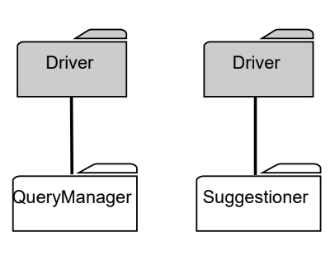
\includegraphics[width=0.5\linewidth]{Integration/firstLayerIntegration.png}
    \caption{First layer integration}
    \label{fig:enter-label}
\end{figure}
As soon as the DB is ready, we can implement the first layer that will focus on the communication with the DB and the creation of suggestions based on data coming from the drivers.

\subsubsection{Second layer}
\begin{figure}[H]
    \centering
    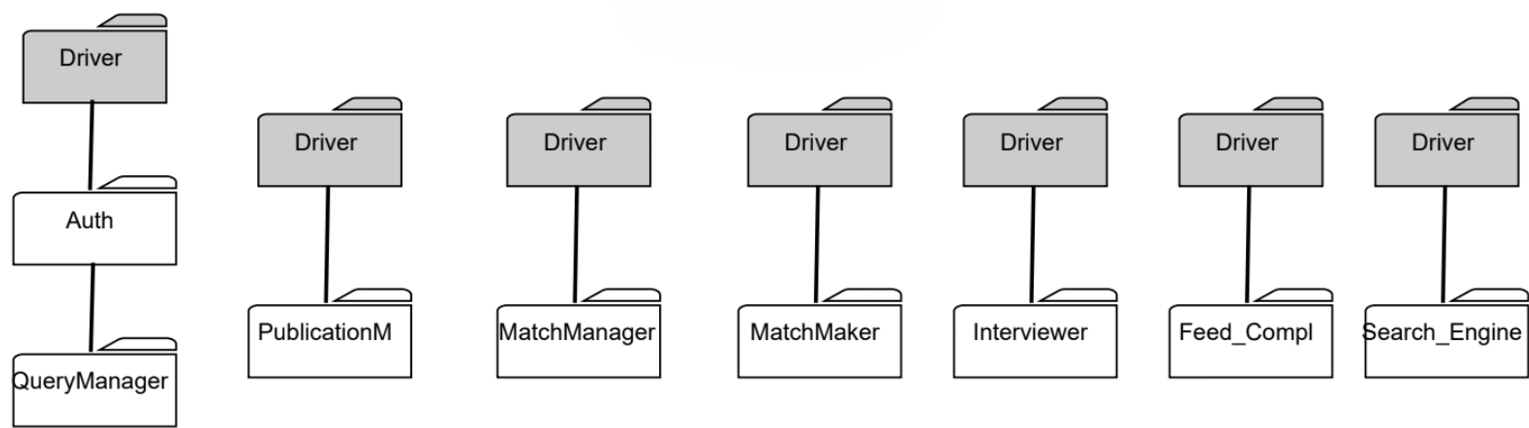
\includegraphics[width=0.5\linewidth]{Integration/secondLayerIntegration.png}
    \caption{Second layer integration}
    \label{fig:enter-label}
\end{figure}
The integration of the second layer allow to test all the basic functions of the system, using a different driver for each component in order to obtain and test the right actions triggered by the right data.

\subsubsection{Intermediate step}
\begin{figure}[H]
    \centering
    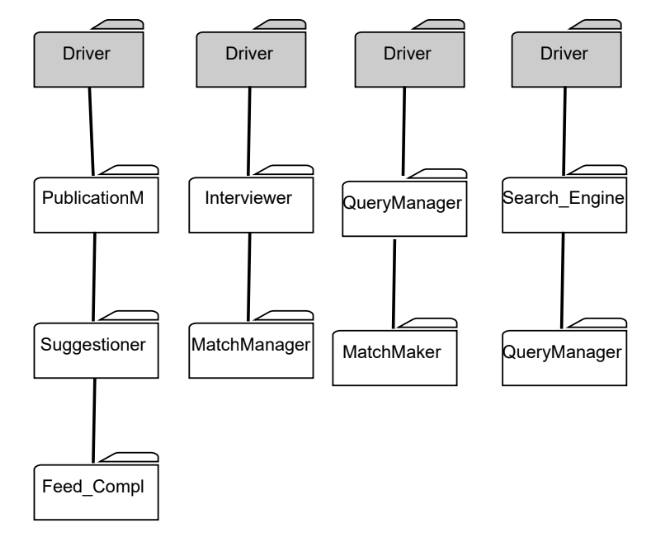
\includegraphics[width=0.5\linewidth]{Integration/intermediateLayerIntegration.png}
    \caption{Intermediate integration step}
    \label{fig:enter-label}
\end{figure}
Before going on with the third layer integration, it's possible to integrate some components in order to test other functions that couldn't have been tested before, like the entire mechanism of creating the CV and internship suggestions or the mechanism of making interviews.

\subsubsection{Third layer}
\begin{figure}[H]
    \centering
    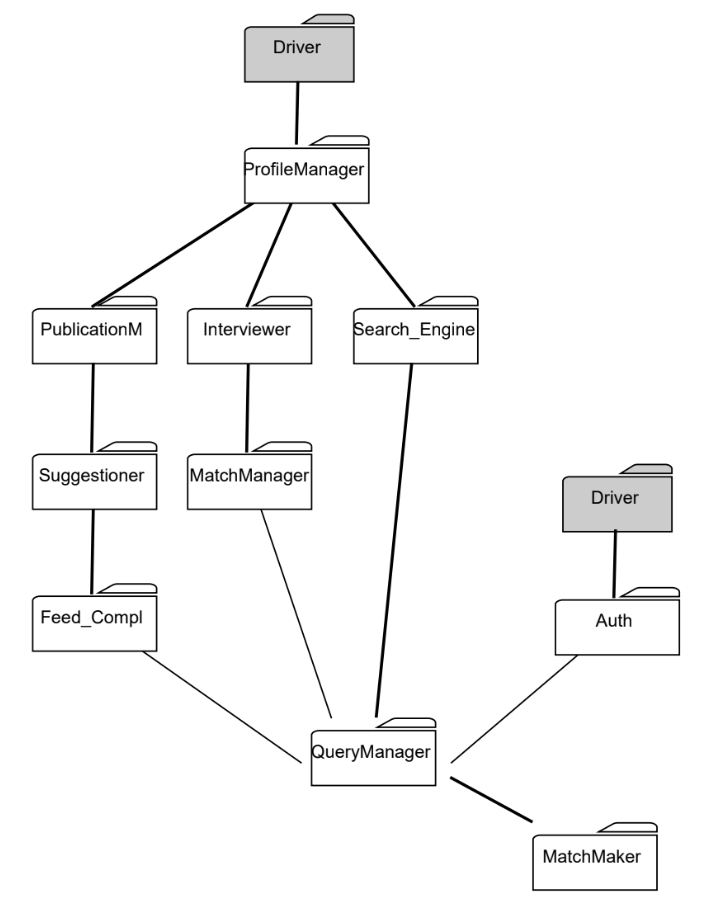
\includegraphics[width=0.5\linewidth]{Integration/ThirdLayerIntegration.png}
    \caption{Third layer integration}
    \label{fig:enter-label}
\end{figure}

This layer is used to integrate the ProfileManager component, allowing to test the remaining part of the system and also to integrate almost all the system with just two drivers.

\subsubsection{Fourth layer}
\begin{figure}[H]
    \centering
    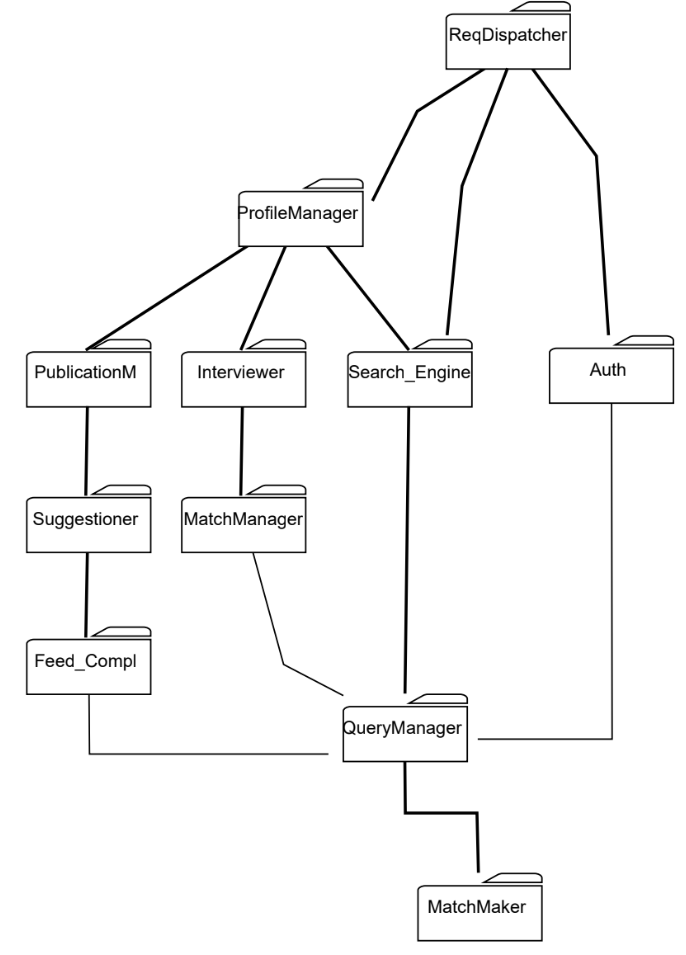
\includegraphics[width=0.5\linewidth]{Integration/FourthLayerIntegration.png}
    \caption{Fourth layer integration}
    \label{fig:enter-label}
\end{figure}
This is the last layer to integrate, RequestDispatcher, the component used to dispatch all the requests from the user. So, integrating this component means all the system is integrated and ready to be tested entirely.

\subsection{Testing Strategy}
To ensure the correctness of the software down to its fundamental components a \textbf{bottom-up} strategy will be adopted.
As soon as a new component is developed and integrated, it is tested to ensure that it works properly. Once all the components have been integrated, an additional series of tests will be done.
In particular:
\begin{itemize}
    \item Functional testing : every functional requirement is tested to hold 
    \item Load testing : The software is meant to be used by a large number of users, making it crucial to ensure its functionality 
\end{itemize}

\section{Effort Spent}
The table below show the number of hours that each member of the group worked for the RASD document.

\begin{table}[H]
    \begin{tabular}{|c|c|}
    \hline
        \textbf{Member}  & \textbf{Hours}\\ 
    \hline
        Elia Priuli &  20h\\
    \hline
        Veronica Viceconti & 21h \\
    \hline
        Marco Zuccoli & 24h \\
    \hline
    \end{tabular}
    \label{tab:my_label}
\end{table}


\section{References}
\begin{enumerate}
    \item Software Engineering II course slides
    \item Draw.io 
    \item Figma to create User Interface Design 
    \item StarUML
\end{enumerate}

\end{document}